\documentclass[11pt,draftcls, onecolumn]{IEEEtran}
\usepackage{graphicx}
\usepackage{amsfonts}
\usepackage{color}
\usepackage[pdftex]{hyperref}
\usepackage{epstopdf}
\usepackage[ruled,vlined]{algorithm2e}
\usepackage{subcaption}
\usepackage{slashbox}
\usepackage{amsmath}
\usepackage{amssymb}
\usepackage{hyperref}
\usepackage{mathrsfs}
\usepackage{latexsym}
\usepackage{multirow}
% \usepackage[caption=false]{subfig}

\ifCLASSOPTIONcompsoc
  \usepackage[nocompress]{cite}
\else
  \usepackage{cite}
\fi


% new command section, Thanks for JMO for the suggestion to keep the document clean and unifited.


% The newcommand file to define the variables

\usepackage{xspace}

\newcommand{\mbf}{\mathbf}
%\DeclareMathOperator*{\argmin}{arg\,min}

\newcommand{\mypartitle}[2][2]{\vspace*{-#1 ex}~\\{\noindent {\bf #2}}}
\newcommand{\mypartitletwo}[1]{\vspace*{-1.5ex}~\\{\noindent \underline{\bf #1}}}

\newcommand{\mycomline}[1]{~\\[0mm]{JMO comment: {\color{blue} #1}}~\\}

\newcommand{\dwucomline}[1]{~\\[0mm]{DWU comment: {\color{red} #1}}~\\}

%%%%%%%%%%%%%%%%%%%%%%%%%%%%%%%%%%%%%%%%%%%%%%%%%
%HMM
%%%%%%%%%%%%%%%%%%%%%%%%%%%%%%%%%%%%%%%%%%%%%%%%%
% random variable
\newcommand{\observation}{\ensuremath{X}\xspace}
\newcommand{\observationSK}{\ensuremath{\observation^{s}}\xspace}
\newcommand{\observationRGBD}{\ensuremath{\observation^{s}}\xspace}
\newcommand{\randomvariable}{$\observation_t$}

% hidden variable
\newcommand{\hiddenstate}{\ensuremath{H}\xspace}
\newcommand{\hiddenstatenode}{\ensuremath{h}\xspace}
\newcommand{\hiddenvariable}{$\hiddenstate_t$}

% finite set
\newcommand{\finiteset}{\ensuremath{\mathcal{H}}\xspace}
% number of hidden states
\newcommand{\numberhiddenstate}{\ensuremath{N_{\finiteset}}\xspace}

% transition matrix
\newcommand{\transitionmatrix}{$p(\hiddenstate_t | \hiddenstate_{t-1})$}

% emission probability
\newcommand{\emissionprob}{\ensuremath{p(\observation_t | \hiddenstate_t)}\xspace}

\newcommand{\emissionprobSK}{\ensuremath{p(X_t^S | H_t)}\xspace}

\newcommand{\emissionprobRGBD}{\ensuremath{p(X_t^R | H_t)}\xspace}
% general input for hmm
\newcommand{\inputhmm}{$x_i$}

% general frame label for hmm
\newcommand{\framelabelhmm}{$y_i$}

% ergodic state
\newcommand{\ergodicstate}{$\mathcal{ES}$}
%%%%%%%%%%%%%%%%%%%%%%%%%%%%%%%%%%%%%%%%%%%%%%%%
% HMM numbers

% number of states associated to an individual gesture
\newcommand{\nsig}{$N_{\mathcal{H}_a}$}
% total number of states
\newcommand{\tns}{$N_{\mathcal{H}}$}

%%%%%%%%%%%%%%%%%%%%%%%%%%%%%%%%%%%%%%%%%%%%%%%%%
%  input
%%%%%%%%%%%%%%%%%%%%%%%%%%%%%%%%%%%%%%%%%%%%%%%%%
% skeleton input
\newcommand{\randomvariableSK}{$\observation_t^s$}
% skeleton high level features
\newcommand{\highSK}{\ensuremath{V^s}\xspace}

% RGBD input
\newcommand{\randomvariableRGBD}{$\observation_t^r$}
%RGBD high level features
\newcommand{\highRGBD}{\ensuremath{V^r}\xspace}

% gesture a
\newcommand{\gesturea}{$\textbf{\emph{a}}$}

% number of joints used
\newcommand{\numberofjoints}{$N_j$}

% skeleton features at time t
\newcommand{\skfeaturet}{$x_t^s$}

% skeleton features
\newcommand{\skfeature}{$f_t$}

% number of hidden state
\newcommand{\numberhiddenstates}{\ensuremath{N_\mathcal{H}}}


% Result section
\newcommand{\jaccardindex}{\ensuremath{J\hspace*{-0.1em}I}\xspace}
\newcommand{\eventaccuracy}{\mbox{\emph{Recognized}}\xspace}
\newcommand{\eventconfused}{\mbox{\emph{Confused}}\xspace}
\newcommand{\eventmissed}{\mbox{\emph{Missed}}\xspace}









\begin{document}

\title{Deep Dynamic Neural Networks for Multimodal Gesture
Segmentation and Recognition}

\author{Di~Wu,
        Lionel~Pigou,
        Pieter-Jan Kindermans,
        Nam~Le,
        Ling~Shao,
        Joni Dambre,
        and~Jean-Marc Odobez
%\IEEEcompsocitemizethanks{\IEEEcompsocthanksitem M. Shell is with the Department
%of Electrical and Computer Engineering, Georgia Institute of Technology, Atlanta,
%GA, 30332.\protect\\
%% note need leading \protect in front of \\ to get a newline within \thanks as
%% \\ is fragile and will error, could use \hfil\break instead.
%E-mail: see http://www.michaelshell.org/contact.html
%\IEEEcompsocthanksitem J. Doe and J. Doe are with Anonymous University.}% <-this % stops an unwanted space
%\thanks{Manuscript received April 19, 2005; revised September 17, 2014.}
}


% The paper headers
\markboth{IEEE TRANSACTIONS ON PATTERN ANALYSIS AND MACHINE INTELLIGENCE, December~2014}%
{Shell \MakeLowercase{\textit{et al.}}: Bare Demo of IEEEtran.cls for Computer Society Journals}


\IEEEtitleabstractindextext{%
\begin{abstract}
This paper describes a novel method called deep dynamic neural networks \emph{(DDNN)} for  multimodal gesture recognition.
A semi-supervised hierarchical dynamic framework is proposed for simultaneous gesture segmentation and recognition taking skeleton, depth and RGB images as input observations.
Unlike the traditional construction of complex handcrafted features, all inputs are learnt by deep neural networks: the skeletal module is modelled by deep belief networks \emph{(DBN)}; the depth and RGB module are modelled by 3D convolutional neural networks \emph{(3DCNN)} to extract high-level spatio-temporal features.
The learned representations are then used for estimating emission probabilities of the hidden Markov models to infer a gesture sequence.
The framework can be easily extended by including an ergodic state to segment and recognise video sequences by a frame-to-frame mechanism, making online segmentation and recognition possible.
This purely data driven approach achieves a score of \textbf{\emph{0.81}} in the ChaLearn LAP gesture spotting challenge. The performance is on par with a variety of the state-of-the-art hand-tuned feature approaches and other learning based methods, opening the doors for using deep learning techniques to explore multimodal time series.

\end{abstract}

% Note that keywords are not normally used for peerreview papers.
\begin{IEEEkeywords}
Deep learning, convolutional neural networks, deep belief networks, hidden Markov models, gesture recognition.
\end{IEEEkeywords}}

\maketitle
\IEEEdisplaynontitleabstractindextext
\IEEEpeerreviewmaketitle
\IEEEraisesectionheading{\section{Introduction}\label{sec:introduction}}

\IEEEPARstart{I}{n} recent years, human action recognition has drawn increasing attention of researchers, primarily due to its potential in areas such as video surveillance, robotics, human-computer interaction, user interface design, and multimedia video retrieval.

Previous works on video-based motion recognition~\cite{liuli,xiantong,diwu2} mainly focused on adapting handcrafted features. % and low-level hand-designed features.
These methods usually have two stages: an optional feature detection stage followed by a feature description stage. Well-known feature detection methods (``interest point detectors") are Harris3D~\cite{laptev2005space}, Cuboids~\cite{dollar2005behavior} and Hessian3D~\cite{hession3d}. For descriptors, popular methods are Cuboids~\cite{scovanner20073}, HOG/HOF~\cite{laptev2005space}, HOG3D~\cite{klaser:inria-00514853} and Extended SURF~\cite{hession3d}.
In recent work of Wang \textit{et al.}~\cite{wang2013dense}, dense trajectories with improved motion based descriptors epitomised the pinnacle of handcrafted features and achieved state-of-the-art results on a variety of ``in the wild" datasets.
Based on the current trends, challenges and interests within the action recognition community, it is to be expected that many successes will follow. However, the very high-dimensional and dense trajectory features usually require the use of advanced dimensionality reduction methods to make them computationally feasible.

Furthermore, as discussed in the evaluation paper of Wang \emph{et al.}~\cite{wang2009evaluation}, no universally best hand-engineered feature exists and the best performing feature descriptor is often dataset dependent. This clearly indicates that the ability to learn dataset specific feature extractors can be highly beneficial.
%In the evaluation paper of Wang \emph{et al.}~\cite{wang2009evaluation}, one interesting finding is that there is no universally best hand-engineered feature for all datasets, suggesting that learning features directly from the dataset itself may be more advantageous.
For this reason, even though handcrafted features have dominated image recognition in previous years, there has been a growing interest in learning low-level and mid-level features, either in supervised, unsupervised, or semi-supervised settings~\cite{taylor2010convolutional,le2011learning,baccouche2005spatio}.
%Albeit the dominant methodology for visual recognition from images and videos relies on hand-crafted features, there has been a growing interest in methods that learn low-level and mid-level features, either in supervised, unsupervised, or semi-supervised settings~\cite{taylor2010convolutional,le2011learning,baccouche2005spatio}.

Due to the recent resurgence of neural networks invoked by Hinton and others~\cite{hinton2006fast}, deep neural architectures serve as an effective solution for extracting high-level features from data.
Deep artificial neural networks have won numerous contests in pattern recognition and representation learning. Schmidhuber~\cite{schmidhuber2014deep} compiled a historical survey compactly summarising relevant works with more than 850 entries of credited works.
From this overview we see that these models have been successfully applied to a plethora of different domains: the GPU-based cuda-convnet~\cite{krizhevsky2012imagenet} classifies 1.2 million high-resolution images into 1000 different classes; multi-column deep neural networks~\cite{ciresan2012multi} achieve near-human performance on the handwritten digits and traffic signs recognition benchmarks; 3D convolutional neural networks~\cite{3dcnn}~\cite{ji20133d} recognise human actions in surveillance videos; deep belief networks combined with hidden Markov models~\cite{mohamed2012acoustic}~\cite{diwucvpr14} for acoustic and skeletal joints modelling outperform the decade-dominating paradigm of Gaussian mixture models in conjunction with hidden Markov models. And recently, Baidu research proposed a DeepSpeech system~\cite{hannun2014deepspeech} that combines a well-optimised recurrent neural network (RNN) training system, achieving the best error rate on noisy speech dataset. In these fields, deep architectures have shown great capacity to discover and extract higher level relevant features.

However, direct and unconstrained learning of complex problems remains difficult, since (i) the amount of required training data increases steeply with the complexity of the prediction model and (ii) training highly complex models with very general learning algorithms is extremely difficult. It is therefore a common practice to restrain the complexity of the model. This is generally done by operating on small patches to reduce the input dimension and diversity~\cite{baccouche2005spatio}, or by training the model in an unsupervised manner~\cite{le2011learning}, or by forcing the model parameters to be identical for different input locations (as in convolutional neural networks~\cite{krizhevsky2012imagenet,ciresan2012multi,3dcnn}).


On the sensor side, due to the immense popularity of Microsoft Kinect~\cite{shotton2011real}~\cite{lingshao2}, there has been a recent interest in developing methods for human gesture and action recognition from 3D skeletal data and depth images.
A number of new datasets~\cite{ICMI,fothergill2012instructing,guyon2012chalearn,wang2012mining} have provided researchers with the opportunity to design novel representations and algorithms, and test them on a much larger number of sequences.
While gesture recognition based on 3D joint positions may seem trivial, it is actually not the case due to several factors. A first one is the high dimensionality and the large amount of variability of the pose space itself.
A second aspect that further complicates the recognition is the segmentation of the different gestures. While in practice segmentation is as important as the recognition, it is an often neglected aspect of the current action recognition research which often assume the availability of segmented inputs~\cite{laptev2005space}~\cite{marszalek09}~\cite{Kuehne11}.

In this paper we aim to address these issues by proposing a data driven system, focusing on analysis of acyclic video sequence labelling problems, \emph{i.e.} video sequences that are non-repetitive as opposed to longer repetitive activities, \textit{e.g.} jogging, walking and running. This paper is an extension of the works of~\cite{diwucvpr14},~\cite{wu2014deep} and~\cite{lio2014deep}.
Within a temporal framework labelling videos in a frame-by-frame
The key contributions can be summarised as follows:
\begin{itemize}
\item A Gaussian-Bernoulli Deep Belief Network is proposed to extracts high-level skeletal joint features and the learned representation is used to estimate the emission probability needed to infer gesture sequences;
\item A 3D Convolutional Neural Network  is proposed to extract features from multiple channel inputs such as depth, RGB images;
\item The proposed temporal framework labels a video sequence in a frame-to-frame mechanism, rendering it possible for online gesture segmentation and recognition.
\item Early and late fusion strategies are investigated within the temporal modelling. The result of both mechanisms show that multiple-channel fusions outperform individual modules.
\end{itemize}

The remainder of this paper is organised as follows. Section II reviews related works for gesture recognition with various temporal models and recent deep learning works for RGB-D data. Section III introduces the formulation of our Deep Dynamic Neural Network model and the intuition behind the high level feature extraction. Section IV details the model implementation. Section V conducts the experimental analysis and Section VI concludes the paper with discussions related to future works.

%%%%%%%%%%%%%%%%%%%%%%%%%%%%%%%%%%%%%%%%%%%%%%%%%%%%%%%%%%
\section{Related Work}

Gesture recognition has drawn increasing attention of researchers, primarily due to its growing potential in areas such as robotics, human-computer interaction and user interface design. Different temporal models have been proposed.
Nowozin and Shotton~\cite{nowozin2012action} proposed the notion of ``action points" to serve as natural temporal anchors of simple human actions using a Hidden Markov Model.
Wang \emph{et al.}~\cite{wang2006hidden} introduced a more elaborated discriminative hidden-state approach for the recognition of human gestures. However, their model relying on only one layer of hidden states might not alone be powerful enough to learn a higher level representation of the data and take advantage of very large corpus. In this paper, we adopt a different approach by focusing on feature learning within a temporal model.

There have been a few works exploring deep learning for action recognition in videos. For instance, Ji \emph{et al.}\cite{ji20133d} proposed using 3D convolutional neural network for automated recognition of human actions in surveillance videos. Their model extracts features from both the spatial and the temporal dimensions by performing 3D convolutions, thereby capturing the motion information encoded in multiple adjacent frames. To further boost the performance, they proposed regularising the outputs with high-level features and combining the predictions of a variety of different models. Taylor \emph{et al.}~\cite{taylor2010convolutional}  also explored 3D convolutional networks for learning spatio-temporal features for videos. The experiments in~\cite{wu2014deep} show that multiple network averaging works better than a single individual network and larger nets  will generally perform better than smaller nets. Providing there is enough data, averaging multi-column nets almost will certainly further improve the performance~\cite{ciresan2012multi}.

However, with advent of Kinect has put more emphasis on RGB-D data.
For instance, the benefits of deep Learning using RGB-D data have been explored for object detection or claudication tasks.
Socher \emph{et al.}~\cite{socher2012convolutional} proposed a single convolutional neural net layer for each modality as inputs to multiple, fixed-tree RNNs in order to compose higher order features for 3D object classification. The single convolutional neural net layer provides useful translational invariance of low level features such as edges and allows parts of an object to be deformable to some extent.
% The pooled filter responses are then give to a recursive neural network to learn compositional features and part interactions.
For addressing Gupta \emph{et al.}~\cite{gupta2014learning} proposed a geocentric embedding for depth images that encodes height above ground and angle with gravity for each pixel in addition to the horizontal disparity.
%The depth image was represented by three channels: horizontal disparity, height above ground and angle with gravity.
This augmented representation allows CNN to learn stronger features than when using disparity (or depth) alone.

The gesture recognition doamin has been stimulated by the collection of large public corpus. In particular, the ChaLearn LAP \cite{chalearnLAP} gesture spotting challenge has collected than 14,000 gestures drawn from a vocabulary of 20 Italian sign gesture categories. The emphasis is on multi-modal automatic learning gestures performed by several different users, with the aim of performing user independent continuous gesture spotting.
Some of the top winning methods in the ChaLearn LAP gesture spotting challenge require a set of complicated handcrafted features for either skeletal input, RGBD input, or both.
For instance, Neveroa \emph{et al.}~\cite{neverova2014multi} proposed a pose descriptor consisting of 7 logical subsets for skeleton features while Monnier \emph{et al.}~\cite{Monnier2014multi} proposed to use 4 types of features for skeleton features (normalised joint positions; joint quaternion angles; Euclidean distances between specific joints; and directed distances between pairs of joints, based on the features proposed by Yao \emph{et al.}~\cite{yao2011does}) and histograms of oriented gradients (HOG) descriptor for RGB-D images around hand regions.
In~\cite{Peng2014multi}, the state-of-the-art dense trajectory~\cite{wang2013dense} handcrafted features are adopted for the RGB module.

There is a gradual trend to learn the features for gesture recognition in videos.
Neveroa \emph{et al.}~\cite{neverova2014multi} presents a multi-scale and multimodal deep network for gesture detection and localisation. Key to their technique is a training strategy that exploits i) careful initialisation of individual modalities and ii) gradual fusion of modalities from strongest to weakest cross-modality structure. One major difference between our proposed method and their works is the treatment of the time factor: fixed length of frames are served as the input of their neural networks for the prediction of the final gesture class. To cope with gestures performed at different speeds, several multi-scale networks are trained. Moreover, the skeleton modules used in their network are sets of ad-hoc hand crafted features.




\section{Model Formulation}
\begin{figure}[t]
  \centering
  % Requires \usepackage{graphicx}
  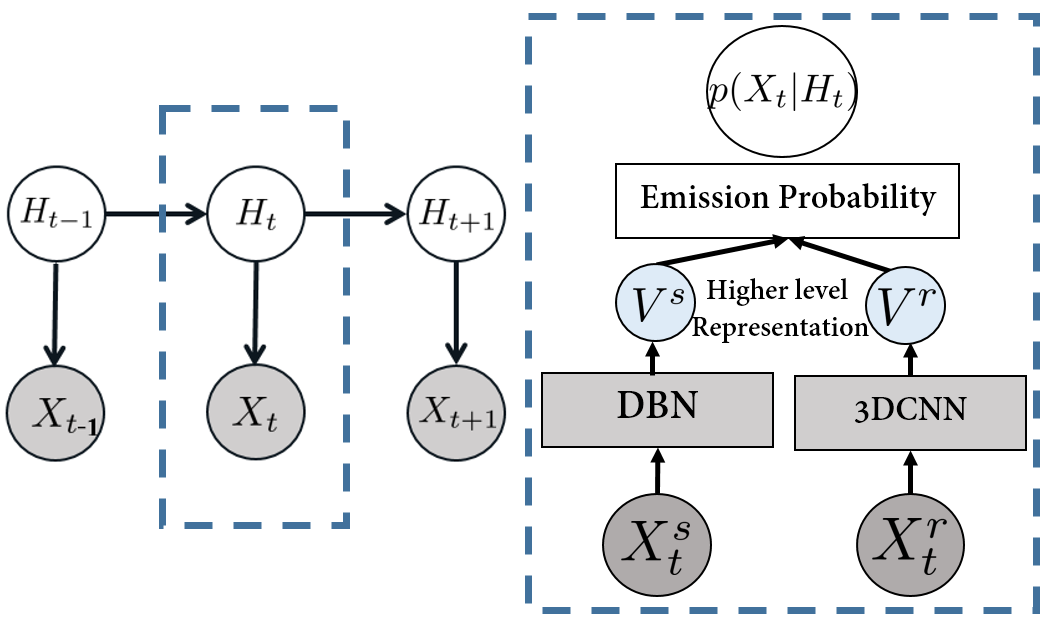
\includegraphics[width=0.48\textwidth]{images/GraphicalModel_new2}\\
  \caption{Per-gesture model: the temporal model is a HMM (left), whose emission probability \emissionprob{} (right) is modeled by a forward-linked chain. The HMM observations \randomvariable{} (skeletal features \randomvariableSK{}, or RGB-D image features \randomvariableRGBD{}) are first passed through deep neural nets: a Deep Belief Network (DBN) for skeletal modality or a 3D convolutional neural network (3DCNN) for the RGB-D modality, to extract high-level features (\highSK{} and \highRGBD{}). The outputs of the neural networks are the emission probabilities of the hidden states $p(X_t | H_t )$.}\label{GM}
\end{figure}
Inspired by the framework successfully applied to speech recognition~\cite{mohamed2012acoustic}, the proposed model is a data driven learning system, relying on a �pure� learning approach. This results in an integrated model, where the amount of prior knowledge and engineering is minimised. On top of that, this approach works without the need for additional complicated preprocessing and dimensionality reduction methods as it is naturally embedded in the framework.

The proposed approach relies on a Hidden Markov Model (HMM) for the temporal part, where the emission probabilities are modelled by two distinctive types of neural networks appropriate for input modality.
 More specifically, the first model works on skeletal features and the neural network for the emission probabilities is a deep boltzmann machine. The second model, on the other hand, uses convolutional neural networks to model the emission probabilities related to RGB and depth (RGBD) video data.
 In the remainder of this section, we will first present our temporal model and then introduce its main component. Details of two distinct neural networks and fusion mechanisms along with post-processing will be provided in Section~\ref{Model Implementation}.


\subsection{Deep Dynamic Neural Networks}\label{Deep Dynamic Neural Networks}
The proposed deep dynamic neural network \emph{(DDNN)} can be seen as an extension of~\cite{diwucvpr14}, where instead of only using the restricted Boltzmann machines to model human motion, various connectivity layers (fully connected layers, convolutional layers) are stacked together to learn higher level features justified by a variational bound~\cite{hinton2006fast} from different input modules.

A continuous-observation HMM with discrete hidden states is adopted for modelling higher level temporal relationships. At each time step $t$, we have one observed random variable \randomvariable{} represents the skeleton input \randomvariableSK{} and RGB-D input \randomvariableRGBD{} as shown in the graphical representation in Fig.~\ref{GM}.
 The unobserved variable \hiddenvariable{} taking on values in a finite set composed of \finiteset{}$=(\bigcup _{a \in \mathcal{A}} \mathcal{H}_a)$, where $\mathcal{H}_a$ is a set of states associated with an individual gesture \gesturea{} related to the different gesture. The unobserved variable \hiddenvariable{} can be interpreted as a segment of a gesture \gesturea{}.

 The intuition motivating this construction is that a gesture is composed of a sequence of poses where the relative duration of each pose may vary. This variance is captured by allowing flexible forward transitions within the chain.
 Classically under the HMM assumption, the joint probability of observations and states is given by:
\begin{equation}
p(H_{1:T},X_{1:T}) = p(H_1)p(X_1 | H_1) \prod^{T}_{t=2} p(X_t | H_t ) p(H_t | H_{t-1}),
\label{HMM_GM_1}
\end{equation}
where $p(H_1)$ is the prior on the first hidden state, \transitionmatrix{} is the transition dynamics modelling the allowed state transitions and their probability and $p(X_t | H_t )$ is the emission probability modelled by the deep neural nets.


%\subsection{Ergodic States Hidden Markov Model}
\begin{figure}[t]
  \centering
  % Requires \usepackage{graphicx}
  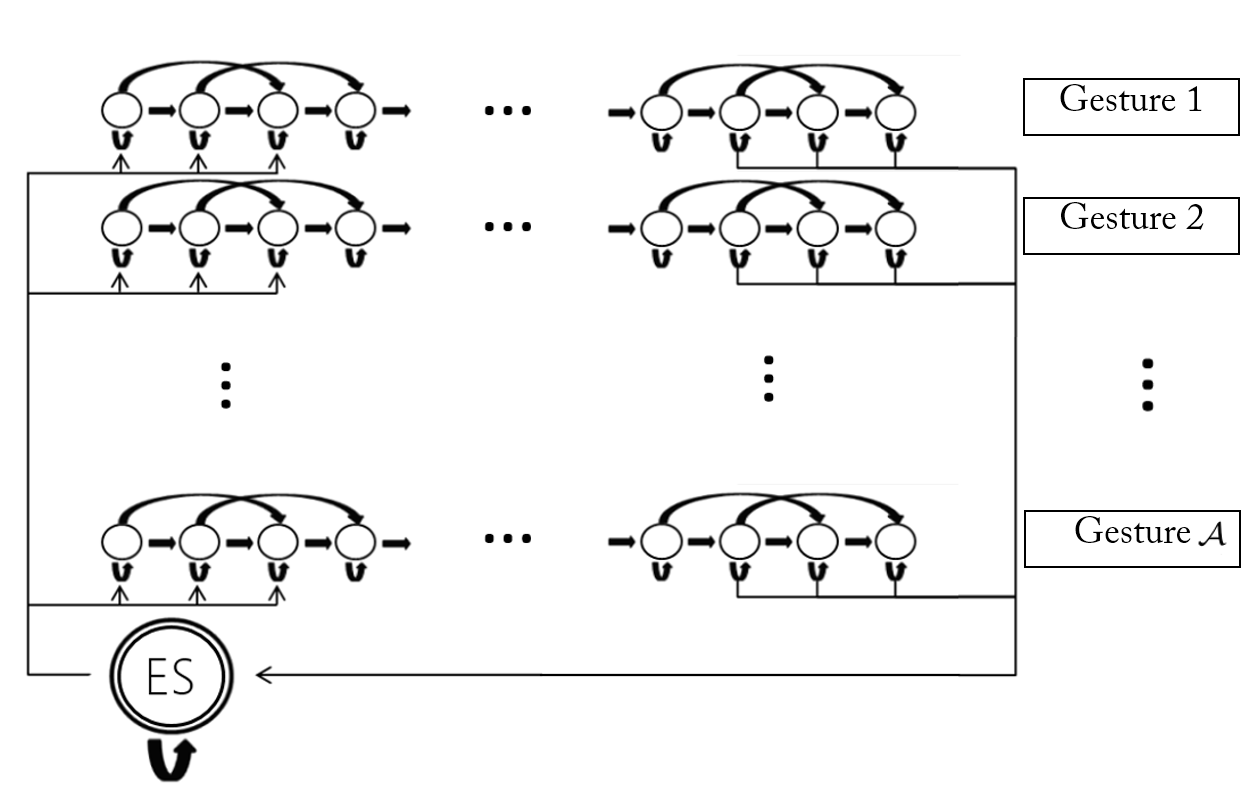
\includegraphics[width=0.48\textwidth]{images/HMM_2_new}\\
  \caption{
    State diagram of the \emph{ES-HMM} model for low-latency gesture segmentation and recognition. An ergodic state (\emph{$\mathcal{ES}$}) is used to model the resting position between gesture sequences. Each node represents a single state and each row represents a single gesture model. The arrows indicate possible transitions between states.}
    \label{HMM_ES}
\end{figure}
The HMM framework can be used for simultaneous gesture segmentation and recognition.
This is achieved by defining the state transition diagram as shown in Fig~\ref{HMM_ES}. For each given gesture $a \in \mathcal{A}$, a set of state $\mathcal{H}_a$ is introduced to defined a Markov model of that gesture. For example, for action sequence ``tennis serving", the action sequence can be dissected into $h_{a_1}, h_{a_2}, h_{a_3}$ as: 1) raising one arm 2) raising the racket 3) hitting the ball.
More precisely, since our goal is to capture the variation in speed of the performed gestures, we set the transition matrix \transitionmatrix{}  in the following way: when being in a particular node $n$ at time $t$, moving to time $t + 1$, we can either stay in the same node (slower), move to node $n + 1$, or move to node $n+2$ (faster).

Further more, to alow segmentation of gesture, we add an ergodic state (\emph{$\mathcal{ES}$}) which resembles the silence state for speech recognition which serve as a catch-all state.
From the $\mathcal{ES}$ we can move to the first three nodes of any gesture class, and from the last three nodes of any gesture class we can move to the $\mathcal{ES}$.
Hence, the hidden variable \hiddenvariable{} can take values within the finite set, defined as $\mathcal{H}=(\bigcup _{a \in \mathcal{A}} \mathcal{H}_a) \bigcup \{\mathcal{ES}\}$, where $\mathcal{ES}$ is the ergodic state as the resting position between gestures. We refer to the model as the ergodic states hidden Markov model (\emph{ES-HMM}) for simultaneously gesture segmentation and recognition.


The \emph{ES-HMM} framework differs from the firing hidden Markov model of~\cite{nowozin2012action} in that we strictly follow a left-right HMM structure without allowing backward transition, forbidding inter-states transverse, assuming that the considered gestures do not undergo cyclic repetitions as in walking for instance.


%The emission probability is represented as a matrix of size $N_{\mathcal{TC}} \times N_{\mathcal{F}}$ where $N_{\mathcal{F}}$ is the number of frames and output target class $N_{\mathcal{TC}}=N_{\mathcal{A}} \times N_{\mathcal{H}_a}+1$ where $N_{\mathcal{A}}$ is the number of gesture classes and $N_{\mathcal{H}_a}$ is the number of states associated to an individual gesture $a$ and one $\mathcal{ES}$ state (\emph{c.f.} Fig. \ref{Sample0700_comparison}: x-axis as $N_{\mathcal{F}}$ and y-axis as $N_{\mathcal{TC}} $ with $\mathcal{ES}$ as the bottom y-axis 101).


Once we have the trained model, we can use standard techniques to infer online the filtering distribution $p(H_t | X_{1:t})$; or offline the smoothed distribution $p(H_t | X_{1:T})$ where $T$ denotes the end of the sequence.
Because the graph for the hidden Markov model is a directed tree, this problem can be solved exactly and efficiently using the max-sum algorithm also known as Viterbi algorithm. This algorithm searches this space of paths efficiently to find the most probable path with a computational cost that grows only linearly with the length of the chain~\cite{bishop2006pattern}.
%We can infer the gesture presence in a new sequence by Viterbi decoding.
% \begin{equation}
%    V_{t,\mathcal{H}}= \log P(X_t | H_t)+  \log(\max_{\mathcal{H} \in \mathcal{H}_a}( V_{t-1,\mathcal{H}}))
%    \label{viterbi_GDBN}
%\end{equation}
%whith the initial state $V_{1,\mathcal{H}}=P(X_1 |H_1)$.
%From the inference results, we define the probability of a gesture $a \in \mathcal{A}$ as $p(y_t=a|x_{1:t}) =V_{T,\mathcal{H}}$.
The result of the Viterbi algorithm is a path--sequence $h_{t:T}$ of nodes going through the state diagram of Fig.\ref{HMM_ES} and from which we can easily infer the class of the gesture as illustrated in Fig. \ref{Sample0700_comparison}.



\subsection{Learning the emission probability \emissionprob{}}\label{Problem formation}

Traditionally, GMMs and HMMs co-evolved as a way of doing speech recognition when computers were too slow to explore more computationally intensive approaches. GMMs are easy to fit when they have diagonal covariance matrices and, with enough components, they can model any distribution. They are, however, statistically inefficient at modeling high-dimensional data that has many kind of componential structure as explained in~\cite{mohamed2012acoustic}. Suppose, for example, that $\mathcal{N}$ significantly different patterns can occur in one sub-band and $\mathcal{M}$ significantly different patterns can occur in another sub-band. Suppose also that which pattern occurs in each sub-band is approximately independent. A GMM requires $\mathcal{N*M}$ components to model this structure because each component must generate both sub-bands(each piece of data has only a single latent cause). On the other hand, a model that explains the data using multiple causes only requires $\mathcal{N+M}$ components, each of which is specific to a particular sub-band. This exponential inefficiency of GMMs for modeling factorial structures leads to the GMMs+HMMs systems that have a very large number of Gaussians, most of which must be estimated from a very small fraction of the data.

The benefit of learning a generative model is greatly magnified when there is a large supply of unlabeled skeletal, RGB and depth data either acquired by motion capture systems or inferred from depth images in addition to the training data that has been labeled by a forced HMM alignment. We do not make use of unlabeled data in this paper, but it could only improve our results relative to purely discriminatively approaches.

Naturally, many of the high-level features learned by the generative model may be irrelevant for making the required discriminations, even though they are important for explaining the input data. However, this is a price worth paying if computation is cheap and high-level features are very good for discriminating between classes of interest.
The benefit of each weight in a neural network being constrained by a larger faction of training case than each parameter in a GMM has been masked by other differences in training. Neural networks have traditionally been training discriminatively, whereas GMMs are typically trained as generative models (even if discriminative training is performed later in the training procedure). Generative training allows the data to impose many more bits of constraints on the parameters, hence partially compensating for the fact that each component of a large GMM must be trained on a very small fraction of the data.

Feed forward neural networks offer several potential advantages over GMMs:
\begin{itemize}
\item Their estimation of the posterior probabilities of HMM states does not require detailed assumptions about the data distribution.
\item They allow an easy way of combining diverse features, including both discrete and continuous features.
\item They use far more of the data to constrain each parameter because the output on each training case is sensitive to a large fraction of the weights.
\end{itemize}
\textbf{Learning the higher level representation for skeleton joints features}: \label{skeleon_high_level}\newline Neal and Hinton~\cite{neal1998view} demonstrated that the negative log probability of a single data vector, $\textbf{v}^0$, under the multi-layer generative model is bounded by a variational free energy, which is the expected energy under the approximating distribution, $Q(\textbf{h}^0 |\textbf{v}^0 )$, minus the entropy of that distribution. For a directed model, the ``energy" of the configuration $\textbf{v}^0 $,$\textbf{h}^0$ is given by $  E(\textbf{v}^0, \textbf{h}^0) = - [ \log p(\textbf{h}^0)+ \log p(\textbf{v}^0 | \textbf{h}^0)]$.
So the bound is
\begin{align*}
    \log p(\textbf{v}^0) &\geqslant \sum_{\textbf{h}^0} Q(\textbf{h}^0 | \textbf{v}^0) [ \log p (\textbf{h}^0) + \log p (\textbf{v}^0 | \textbf{h}^0)] \\
     &- \sum_{\textbf{h}^0} Q(\textbf{h}^0 | \textbf{v}^0) \log Q(\textbf{h}^0 |\textbf{v}^0)
\end{align*}

The intuition using deep belief networks for modeling marginal distribution \emissionprob{} in skeleton joints action recognition is that by constructing multi-layer networks, semantically meaningful high level features for skeleton configuration will be extracted whilst learning the parametric prior of human pose from mass pool of skeleton joints data. In the recent work of~\cite{6751269} a non-parametric bayesian network is adopted for human pose prior estimation, whereas in our framework, the parametric networks are incorporated.

Using the pair wise joints features as raw input, the data-driven approach network will be able to extract relational multi-joints features which are relevant to target frame class. E.g., for ``toss" action, wrist joints is rotating around shoulder joints would be extracted from the backpropagation via target frame as those task specific, \emph{ad hoc} hard wired sets of joints configurations as in~\cite{chaudhry2013bio}~\cite{muller2006motion}\cite{nowozin2012action}~\cite{ofli2013sequence}.

The outputs of the neural net are the hidden states learned by force alignment during the supervised training process.
Once we have model, we can use the normal online or offline smoothing, inferring the hidden marginal distributions of every node (frame) of the test video.

The overall algorithm for training and testing are presented in Algorithm \ref{MMDDN_train} and \ref{MMDDN_test}.

\begin{algorithm}
\caption{Multimodal deep dynamic networks -- training}\label{MMDDN_train}
\LinesNumbered
\SetAlgoLined
\SetAlgoNoEnd
\DontPrintSemicolon
\SetKwFunction{zeroes}{zeroes}
\KwData{\;
          \inputhmm{}=$[x_{i,1}, \ldots,x_{i,t},\ldots, x_{i,T}]$ \;
          $ \mathbf{X^1=\{ x^1_i\}_{i \in [1 \ldots t]}}$ - raw input (skeletal) feature \; \hspace{1cm} sequence.\;
          $ \mathbf{X^2=\{ x^2_i\}_{i \in [1 \ldots t]}}$ - raw input (depth) feature \; \hspace{1cm} sequence in the form of     $M_1 \times M_2 \times T$, where \; \hspace{1cm} $M_1, M_2$ are the height and width of the input \; \hspace{1cm} image and $T$  is the number of contiguous \; \hspace{1cm} frames of the spatio-temporal cuboid. \;
          $ \mathbf{Y=\{ y_i\}_{i \in [1 \ldots t]}}$  - frame based local label (achieved by\; \hspace{1cm} semi-supervised forced-aligment), where \;
          \hspace{1cm} $ \mathbf{y_i} \in \{ N_{\mathcal{A}} * N_{\mathcal{H}_a} + \textbf{\emph{1}} \} $ with $N_{\mathcal{A}}$ the number of \;
          %\hspace{1cm} classes, $N_{\mathcal{H}_a$ is the number of hidden states for \; \hspace{1cm} each class,
          \hspace{1cm} gesture classes and $N_{\mathcal{H}_a}$ is the number of \;
          \hspace{1cm} states associated to an individual gesture $a$ \;
          \hspace{1cm} and $\textbf{\emph{1}}$ as ergodic state.
            }
%\For{$m \leftarrow 1$ to $2$}{
    \SetAlgoVlined
    %\eIf{$m$ is $1$}{


        Preprocess skeletal data $ \mathbf{X^1}$ as in Eq.\ref{sk_features_1}, \ref{sk_features_2}, \ref{sk_features_3}.\;
        Normalise (zero mean, unit variance per dimension) the above features and feed it to Eq.\ref{GRBMenergy}. \;
        Pre-train the networks using \emph{Contrastive Divergence}. \;
        Supervised fine-tuning of the deep belief networks using $ \mathbf{Y}$ by standard mini-batch \emph{SGD} backpropagation.\;
    %}{
        Preprocess the depth and RGB data $ \mathbf{X^2}$ as in \ref{3d_preproc}.\;
        Feed the above features to Eq.\ref{ReLU}. \;
        Train the 3D convolutional neural networks using $ \mathbf{Y}$.\;
    %}
%}
\KwResult{\;
        $\mathbf{GDBN}$ - a Gaussian-Bernoulli visible layer deep \;
                \hspace{1cm} belief network to generate the emission \;
                \hspace{1cm} probabilities for the hidden Markov model.\;
        $\mathbf{3DCNN}$ - a 3D deep convolutional neural \;
                    \hspace{1cm} network to generate the emission probabilities\;
                    \hspace{1cm} for the hidden Markov model.\;
        $\mathbf{p(X_t | H_t )}$ emission probability. \;
        $\mathbf{p(H_1)}$ - prior probability for $ \mathbf{Y}$ by accumulating and \;
                \hspace{1cm} normalising labels.\;
        $ \mathbf{p(H_t | H_{t-1})}$ - transition probability for $ \mathbf{Y}$,  enforcing\;
                \hspace{1cm} the beginning and ending of a sequence can \;
                \hspace{1cm} only start from the first or the last state.
}
\end{algorithm}
%%%%%%%%%%%%%%%%%%%%%%%%%%%%%%%%%%%%%%%%%%%%%%%%%%%%%%%%%%%%%%%%%%%%%%%%%%%%%%%%%%%%%%%%%%%%%%%%%%%%%%%%%%%%%%%%
\begin{algorithm}[t]
\caption{Multimodal deep dynamic networks -- testing}\label{MMDDN_test}
\LinesNumbered
\SetAlgoLined
\SetAlgoNoEnd
\DontPrintSemicolon
\SetKwFunction{zeroes}{zeroes}
\KwData{\;
         $\mathbf{X^1=\{x^1_i\}_{i \in [1 \ldots t]}}$ - raw input (skeletal) feature \; \hspace{1cm} sequence.\;
         $\mathbf{X^2=\{x^2_i\}_{i \in [1 \ldots t]}}$ - raw input (depth) feature \; \hspace{1cm} sequencein the form of $M_1 \times M_2 \times T$. \;
         $\mathbf{GDBN}$ - trained Gaussian-Bernoulli visible layer  \;
                \hspace{1cm} deep belief network to  generate the emission\;
                 \hspace{1cm} probabilities for the hidden Markov model.\;
         $\mathbf{3DCNN}$ - trained  3D deep convolutional neural\;
                    \hspace{1cm} network to generate the emission\;
                    \hspace{1cm} probabilities for the hidden Markov model.\;
        $\mathbf{p(H_1)}$ - prior probability for $ \mathbf{Y}$.\;
        $ \mathbf{p(H_t | H_{t-1})}$ - transition probability for $ \mathbf{Y}.$
            }

%\For{$m \leftarrow 1$ to $2$}{
    \SetAlgoVlined
    %\eIf{$m$ is $1$}{
        Preprocessing and normalising the skeletal data $ \mathbf{X^1}$  as in Eq. \ref{sk_features_1}, \ref{sk_features_2}, \ref{sk_features_3}.\;
        Feedforwarding network $\mathbf{GDBN}$ to generate the emission probability $\mathbf{p(X_t | H_t )}$ in Eq.\ref{HMM_GM_1}. \;
        Generating the score probability matrix $\mathbf{S^1 = p(H_{1:T},X_{1:T}).}$ \;
    %}{
        Preprocessing(median filtering the depth data) and normalising data RGBD data $ \mathbf{X^2}$ .\;
        Feedforwarding $\mathbf{3DCNN}$ to generate the emission probability $\mathbf{S^2 = p(X_t | H_t )}$ in Eq.\ref{HMM_GM_1}. \;
        Generating the score probability matrix $\mathbf{S^2 =p(H_{1:T},X_{1:T}).}$ \;
    %}
%}
        Fuse the score matrix $\mathbf{S = \alpha * S^1 + (1-\alpha)* S^2}$ OR the learnt joint representation.\;
        Finding the best path $\mathbf{V_{t,\mathcal{H}}}$ using $\mathbf{S}$ by Viterbi decoding as in Eq.\ref{viterbi_GDBN}. \;
\KwResult{\;
        $ \mathbf{Y=\{ y_i\}_{i \in [1 \ldots t]}}$  - frame based local label  \;
        $ \mathbf{C}$ - global label, the anchor point is chosen as the\;
                        \hspace{1cm} middle state frame.\;
}
\end{algorithm}


\section{Model Implementation}\label{Model Implementation}
In this section, we detail the proposed Deep Dynamic Neural Networks and its individual composition implementations.
\subsection{Ergodic States Hidden Markov Model}
 In all our experiments, the different modelling elements are specified as follows: the number of states \nsig{} associated to an individual gesture has been set to 5. Therefore, in total, the number of  \tns{}$= 20(classes) \times 5 + 1 = 101$ as experiments are conducted on the Chalearn dataset.
 The training data in Chalearn is given as a set of sequences \inputhmm{}=$[x_{i,1}, \ldots,x_{i,t},\ldots, x_{i,T}]$ where $x_{i,t}=[x_{i,t}^s, x_{i,t}^r]$ corresponds to the skeleton and RGB-D input. As the gesture label is provided for each sequence, we need to define \framelabelhmm{}=$[y_{i,1}, \ldots,y_{i,t},\ldots, y_{i,T}]$, the sequence of state labels $y_{i,t}$ associated to each frame. To do so, a force alignment is used which means that if the $i^{th}$ sequence is a gesture \gesturea{}, then the first $\lfloor \frac{T_i}{5} \rfloor$ frames are assigned to state $h_a^1$ (the first state of gesture \gesturea{}), the following $\lfloor \frac{T_i}{5} \rfloor$ frames are assigned to $h_a^2$, and so forth.
Note that each gesture sequence comes with the video frames proceeding and following the gesture. In practice, we dictate 5 frames before and after each gesture sequence and labelled this shot sequence with the ergodic state (\ergodicstate{}) label.
Transitional matrix \transitionmatrix{} is collected from the statistics of labelling stage, allowing 5 frame jumps to accommodate skipping states.

% \begin{flushleft}
%\textbf{\emph{Hidden states} ($\mathcal{H}_a$): } Force alignment is used to extract the hidden states, \emph{i.e.} if a gesture token is 100 frames, the first $20= \frac{100}{5(N_{\mathcal{H}_a} )}$ frames are assigned to hidden state $\textbf{\emph{1}}$, the following 20 frames are assigned to hidden state $\textbf{\emph{2}}$, and so forth.
%
%\textbf{\emph{Ergodic states ($\mathcal{ES}$)}:} Neutral frames are extracted as 5 frames before or after a gesture token, according to the ground truth labels.
%
%\textbf{\emph{Transitional Matrix (\transitionmatrix{})}:} Statistics is collected from the labelling stage, allowing 5 frame jumps to accommodate skipping states.
%\end{flushleft}
\subsection{Skeleton Module}
\begin{figure}[t]
  \centering
  % Requires \usepackage{graphicx}
  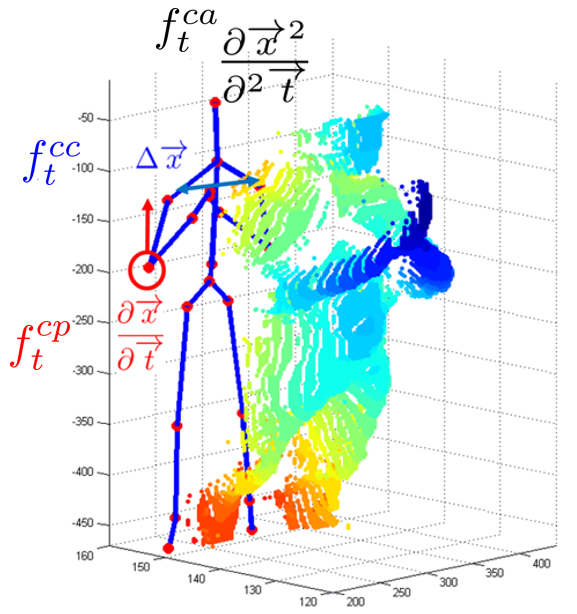
\includegraphics[width=0.3\textwidth]{images/point_cloud}\\
  \caption{
    A point cloud projection of a depth image and the 3D positional features.}
    \label{point_cloud}
\end{figure}




%\subsubsection{Preprocessing}
Given our task, only upper body joints are relevant. Accordingly, only the \numberofjoints{}$ =11$ upper body joints are considered, namely \emph{``ElbowLeft, WristLeft, ShoulderLeft, HandLeft, ElbowRight, WristRight, ShoulderRight, HandRight, Head, Spine, HipCenter"}.

Skeleton features of time $t$ are defined as \skfeaturet{}$=x_t^{s,1}, \ldots, x_t^{s, N_j}$. To capture the gesture dynamics, rather than using \skfeaturet{} as raw input to our data drive approach, we follow the features used in~\cite{diwucvpr14} and compute 3D positional pairwise differences of joints as well as temporal derivatives, defined as (as shown in Fig. \ref{point_cloud}) \footnote{Note that offset features used in~\cite{diwucvpr14} depends on the first frame, if the initialisation fails which is a very common scenario, the feature descriptor will be generally very noisy. Hence, the offset features are discarded and only the three more robust features $[f^{cc}_t, f^{cp}_t, f^{ca}_t]$}:
\begin{align}
f^{cc}_t&=\{x_t^{s,i}-x_t^{s,j} | i,j=1,2,\ldots, N_j; i\neq j\} \label{sk_features_1}\\
f^{cp}_t&=\{x_{t+1}^{s,i}-x_t^{s,i} |  i=1,2,\ldots, N_j\} \label{sk_features_2}\\
f^{ca}_t&=\{x_{t+1}^{s,i} - 2 \times x_t^{s,i} + x_t^{s,i} | i=1,2,\ldots, N_j  \} \label{sk_features_3}
\end{align}


This results in an input feature $f_t=[f^{cc}_t, f^{cp}_t, f^{ca}_t]$ of dimension $N_f=N_j \times( \frac{ N_j}{2} + N_j + N_j)*\mathit{3}=891$.
Admittedly, here we do not completely neglect human prior knowledge about information extraction for relevant static postures, velocity and acceleration of overall dynamics of motion data.
While we have indeed used prior knowledge to define our relevant features, we believe they remain quite general and do not need data-set specific tuning.
Note that feature extraction process resembles the computation of \emph{Mel Frequency Cepstral Coefficients (MFCCs)} and their temporal derivatives for the speech recognition community~\cite{mohamed2012acoustic}.
%\textbf{\emph{Caveat}}:
%\begin{itemize}
%\item  When extracting skeletal features, the 3D joint coordinates have not been transformed from the world coordinate system to a person centric coordinate system by placing the \emph{``HipCenter"} at the origin.
%\item  Note also that the normalization scheme by scaling the skeleton position using length of \emph{``HipCenter"} and \emph{``Spine"} didn't work well in the implementation.
%\item The third point worth noting is that some actors performed gestures using left hand as a dominant hand whereas some using right hand which worth investigating the effect of this in the future. However, those tokens are treated indiscriminately.  Hence, the feature fed into \emph{GRBM} are almost raw, un-preprocessed.
%\end{itemize}

\subsubsection{Modeling \randomvariableSK{} using Deep Belief Networks}

Once we have the skeleton input feature \skfeature{} which served as the input \randomvariableSK{} for DBN in Fig.~\ref{GM}. The emission probability \emissionprob{} can be generated using a Deep Belief Networks. We briefly introduce the building elements of the network and a more detailed introduction can be found at~\cite{salakhutdinov2009learning}:
  

Boltzmann Machines (BMs) are a special structure of Markov Random Field (MRF), \emph{i.e.} the energy function is linear in term of its corresponding free parameters.
To empower the expressiveness of the model so as to encode complex distributions, the hidden variables are introduced to enhance the modelling capability of the Boltzmann Machines

Restricted Boltzmann Machines (RBMs) is a subtype of BMs in that there is no connections between visible to visible or hidden to hidden variables. RBM, as a special type of Markov random field with a two-layer structure, has the visible binary stochastic units $v\in \{0,1\}^D$ connected to the hidden binary stochastic units $h\in \{0,1\}^F$. 

The energy of the state $\{v,h\}$is:
\begin{eqnarray}
E(v,h;\theta)&=&-v ^{\top}Wh-b^{\top}v-a^{\top}h  \\
             &=&-\sum^D_{i=1} \sum^F_{j=1} W_{ij} v_i h_j -\sum^D_{i=1}b_iv_i - \sum^F_{j=1}a_jh_j
   \label{energy}
\end{eqnarray}
where $\theta=\{W,b,a\}$ are the free parameters: $W_{i,j}$ serves as the symmetric synergy term between visible unit $i$ and hidden unit $j$; $b_i$ is the bias term of the visible units and $a_j$ is the bias term of the hidden units. The joint distribution over the visible and hidden units is defined by:
\begin{eqnarray}
    P(v,h;\theta)&=&\frac{1}{Z(\theta)} \exp(-E(v,h;\theta)); \\
        Z(\theta)&=&\sum_v \sum_h exp(-E(v,h;\theta))
    \label{RBM}
\end{eqnarray}
The conditional distributions needed for inference and generation are given by:
\begin{eqnarray}
    P(h_{j=1}|\textbf{v})&=&g(\sum_i W_{ij}v_i+a_j)); \\
      P(v_{i=1}|\textbf{h})&=&g(\sum_j W_{ij}h_j+b_i))
\end{eqnarray}
where $g(x)=\frac{1}{1+exp(-x)}$ is the logistic function.

The derivative of the log-likelihood with respect to the model parameter from Eq.~\ref{RBM} is expressed as: $E_{P_{data}}[vh^{\top}]-E_{P_{model}}[vh^{\top}]$ where $E$ denotes the expectation.
Due to the intractability of the second term, an approximation is generally required. This approximation is called the ``Constrative Divergence":
%In practice, learning is done by following an approximation to the gradient of a different objective function, called the ``Constrative Divergence":
\begin{equation}
    \Delta W = \alpha (E_{P_{data}}  [\textbf{vh}^T]-E_{P_T}[\textbf{vh}^T]). \label{CD1}
\end{equation}
where $\alpha$ is the learning rate and $P_T$ is the distribution obtained by running a Gibbs chain, initialized with the visible units given by the data, for $T$ full steps.

Because input skeletal features \skfeature{} are continuous instead of binomial features, we use the Gaussian-Bernoulli RBM (\emph{GRBM}) to model the energy term of first layer. More precisely:
\begin{equation}
    E(v,h;\theta) =-\sum^D_{i=1} \frac{(v_i-b_i)^2}{2\sigma_i^2} -\sum^D_{i=1} \sum^F_{j=1} W_{ij}  h_j \frac{v_i}{\sigma_i}- \sum^F_{j=1}a_jh_j
\label{GRBMenergy}
\end{equation}

The conditional distributions needed for inference and generation are given by:
\begin{equation}
    P(h_{j=1}|\textbf{v})=g(\sum_i W_{ij}v_i+a_j));
\end{equation}
\begin{equation}
    P(v_{i=1}|\textbf{h})=\mathscr{N}(v_i|\mu_i,\sigma_i^2).
\end{equation}
where $\mu_i=b_i+\sigma_i^2 \sum_j W_{ij} h_j$ and $\mathscr{N}$ is the normal distribution. In general, we normalise the data (mean substraction and standard deviation division) in the preprocessing phase. Hence, in practice, instead of learning $\sigma_i^2$, one would typically use a fixed, predetermined unit value $\textbf{\emph{1}}$ for $\sigma_i^2$.

\begin{figure}[t]
  \centering
  % Requires \usepackage{graphicx}
  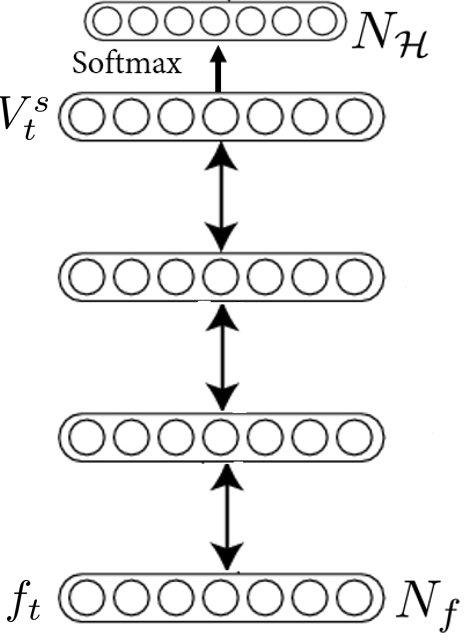
\includegraphics[width=0.25\textwidth]{images/DBN}\\
  \caption{
    Deep Belief Network using skeleton input \skfeature{} to predict emission probability \emissionprob{}.}
    \label{DBN}
\end{figure}

By stacking a softmax layer on top of the RBMs as in Fig.~\ref{DBN}, a Deep Belief Network is built for predicting emission probability \emissionprob{}. The weights are fine-tuned slightly from the top.

For high-level skeleton feature extraction, the network architectures is $[N_f,2000,2000,1000,N_{\mathcal{H}}]$,
 where $N_f = 891$ is the observation domain dimensionality; $N_{\mathcal{H}}$ is the output target class.






 In the training set, there are in total $400\,117$ frames. During the training of the \emph{DBN}, $90\%$ is used for training, $8\%$ for validation (for the purpose of early stopping) $2\%$ is used for test evaluation.
The feed forward networks are pre-trained with a fixed recipe using stochastic gradient decent with a mini-batch size of 200 training cases. Unsupervised initialisations (we run 100 epochs for unsupervised pre-training) tend to avoid suboptimal local minima and increase the network�s performance stability. For Gaussian-Bernoulli RBMs, the learning rate is fixed at 0.001 while for binary-binary RBMs the learning is 0.01 (note that in general, training \emph{GRBMs} requires smaller learning rates). For fine-tuning, the learning rate starts at 1 with 0.99999 mini-batch scaling. During the experiments, early stopping occurs around epoch 440.
The optimisation completes with a frame based validation error rate of $16.5\%$, with $16.15\%$ on the test set. The frame based validation error rate is shown in Fig~\ref{sk_error_rate} .

% Although that further optimising the network architecture would lead to more competitive results, in order not to overfit, ``as algorithms over time become too adapted to the data set, essentially memorising all its idiosyncrasies, and losing ability to generalise"~\cite{torralba2011unbiased}, we would like to treat the model as the aforementioned more generic approach.
% Since a completely new approach will initially have a hard time competing against established, carefully fine-tuned methods.
%More fundamentally, it may be that the right way to treat dataset performance numbers is not as a competition for the top place.
%This way, fundamentally new approaches will not be forced to compete for top performance right away, but will have a chance to develop and mature.
The performance of the skeleton module is shown in Tab.~\ref{Table_score_fusion}.

\begin{figure}[t]
  \centering
  % Requires \usepackage{graphicx}
  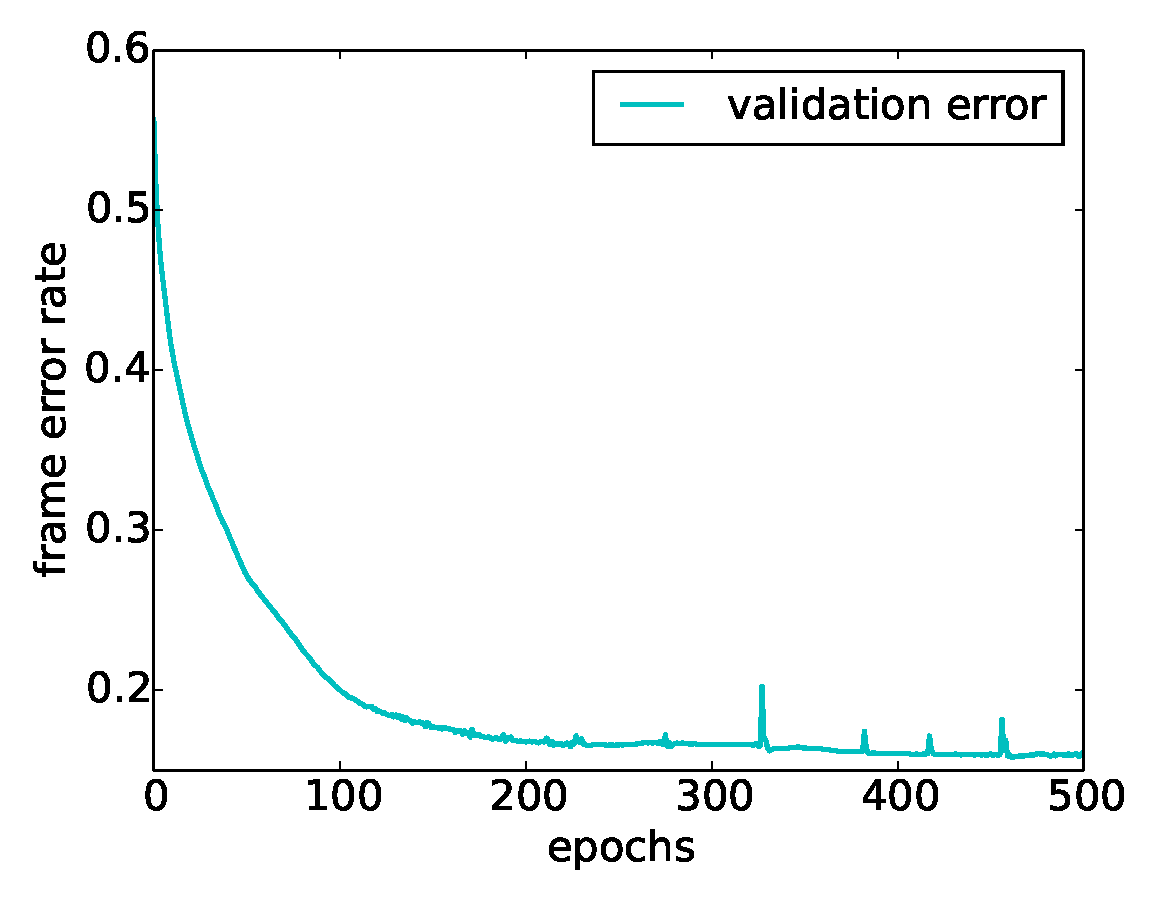
\includegraphics[width=0.4\textwidth]{images/training_error_sk}\\
  \caption{
    Deep belief network frame based validation error rate for the skeleton input module. The 0.05 frame error rate indicates the well generalisation Deep Belief Network of skeleton modules.}
    \label{sk_error_rate}
\end{figure}

\subsection{RGB \& Depth 3D Module}
\subsubsection{Preprocessing}\label{3d_preproc}

Although DeepMind technology~\cite{mnih2013playing} presented the first deep learning model to successfully learn control policies directly from high-dimensional sensory input using deep reinforcement learning, working directly with raw input Kinect recorded data frames, which are $640 \times 480$ pixel images, can be computationally demanding. 
Therefore, our first step in the preprocessing stage consists of cropping the highest hand and the upper body using the given joint information. In the Chalearn dataset, we determined that the highest hand is the most interesting. When both hands are used, they normally perform the same (mirrored) movement, and when one hand is used, it is always the highest one which is relevant.
Furthermore, to be invariant to handiness, we train the model with the right hand view. That is, when the left hand is actually the performing hand, the video was mirrored.


The preprocessing results in four video samples (body and hand with grayscale and depth) of resolution $64\times64$. Furthermore, the noise in the depth maps is reduced by thresholding, background removal using the user index, and median filtering. 
The depth images are normalised with mean substraction for each image because the median of depth images are irrelevant to the gesture subclass. And both RGB and depth images are normalised by dividing the standard deviation of each image.
The outcome is illustrated in Fig.~\ref{3dcnn input}.
\begin{figure}[t]
  \centering
  % Requires \usepackage{graphicx}
  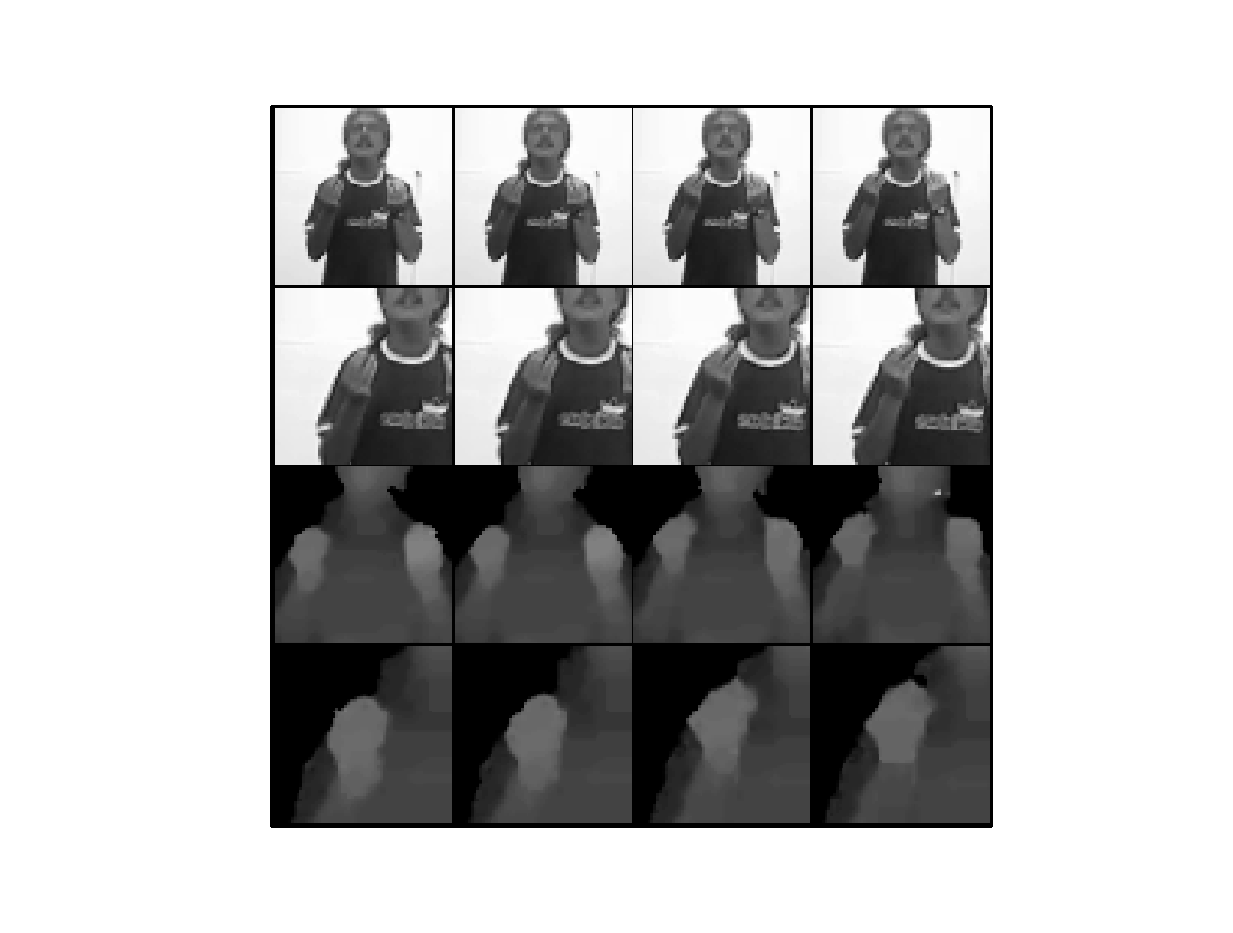
\includegraphics[width=0.5\textwidth]{images/3dcnn_filters/original.eps}\\
  \caption{
    Preprocessing result. Inputs  from top to bottom: 1) grayscale body input, 2) grayscale hand input, 3) depth body input, 4) depth hand input. }
    \label{3dcnn input}
\end{figure}


\subsubsection{3DCNN Architecture}
\begin{figure*}[t]
  \centering
  % Requires \usepackage{graphicx}
  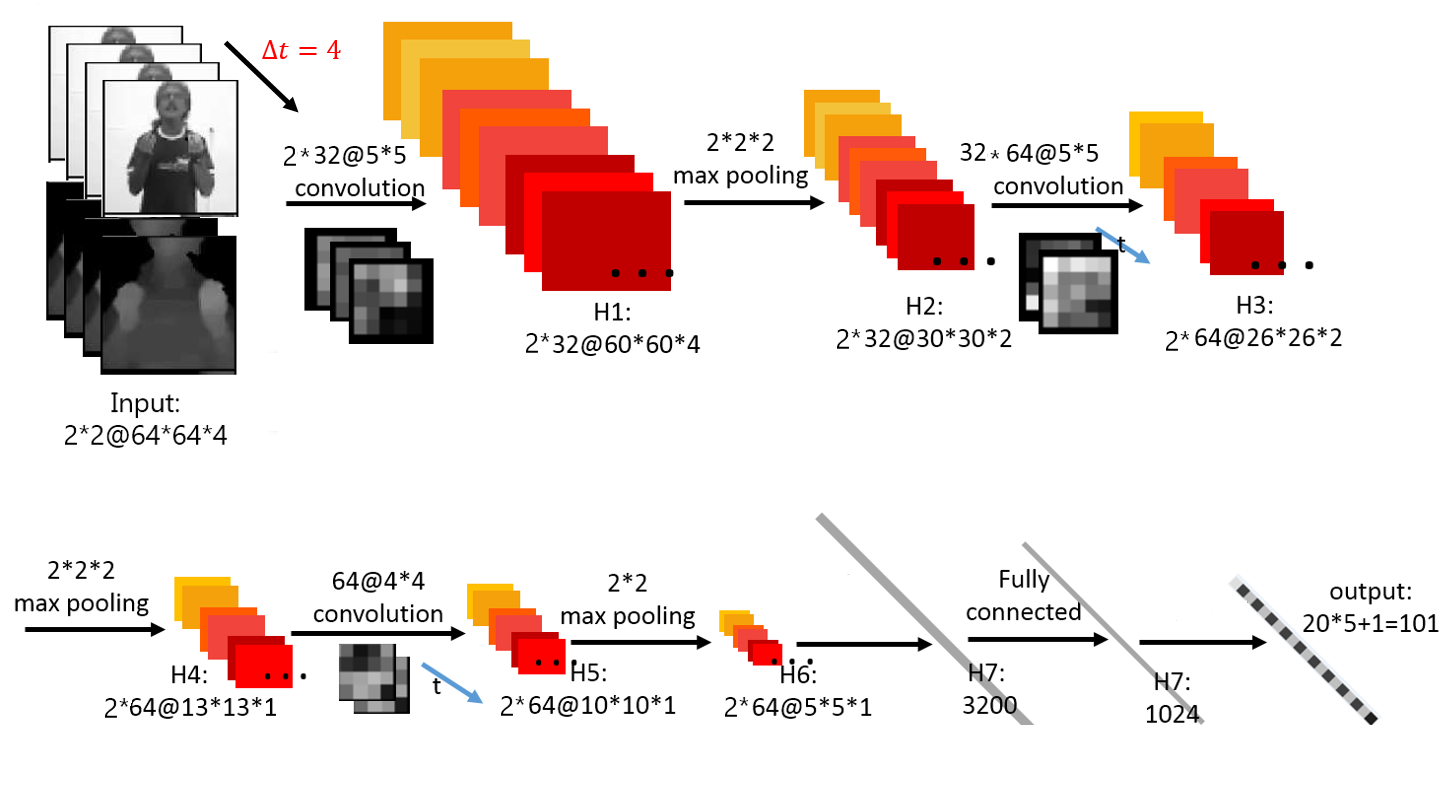
\includegraphics[width=.9\textwidth]{images/3DCNN_new}
  \caption{An illustration of the architecture of the 3DCNN architecture. The 3rd dimension of the input is time with 4 frames stacked together. The depth and RGB data are stacked (concatenated) together at Input. Hand and body part output are concatenated at H7.}\label{3dcnn_architecture}
\end{figure*}

This deep neural network architecture consists of a series of layers composed of either convolution, pooling or, in the last layer, fully connected layers.
The 3D convolution itself is achieved by convolving a 3D kernel to the cuboid formed by stacking multiple contiguous frames together. We follow the nomenclature as in~\cite{ji20133d}.
 However, instead of using $tanh$ units as in~\cite{ji20133d},  Rectified Linear Units (\emph{ReLUs})~\cite{krizhevsky2012imagenet} were used in order to speed up training.
 Formally, the value of a unit at position $(x, y, z)$ ($z$ here corresponds to the time-axis) in the $j$-th feature map in the $i$-th layer, denoted as $v^{xyz}_{ij}$, is given by:
\begin{equation}
v^{xyz}_{ij} =  max( 0,  ( b_{ij} + \sum_m \sum_{p=0}^{P_i - 1} \sum_{q=0}^{Q_i -1 } \sum_{r=0}^{R_i -1} w^{pqr}_{ijm} v^{(x+p)(y+q)(t+r)}_{(i-1)m} ))
\label{ReLU}
\end{equation}

The complete 3DCNN architecture is depicted in Fig.~\ref{3dcnn_architecture} : 4 types~(Fig.~\ref{3dcnn input}) of input contextual frames are stacked as size $64\times64\times4$. 
The first layer consists of 32 feature maps produced by $5\times5$ spatial convolutional kernels followed by local contrast normalisation (LCN)~\cite{jarrett2009best} and 3D max pooling with strides $(2,2,2)$, then the grayscale channel and depth channel are concatenated. The second layer has 64 feature maps with $5\times5$ kernels followed by LCN and 3D max pooling with strides $(2,2,2)$. The third layer is composed of 64 feature maps with $4\times4$ kernels followed by 3D max pooling with strides $(1,2,2)$. All convolutional layer outputs are flattened with the body channel and hand channel concatenated, and fed into one fully connected layer of size $1024$. The output layer has \numberhiddenstates{} values, the number of states in the HMM.
 is of size $ 101 = 5\times20+1$ (number of hidden states for each class $\times$ number of classes plus one ergodic state).




\subsubsection{Details of Learning}
% The first 650 batches are used for training and the remaining 50 files for validation.
During training, dropout \cite{hinton2012improving} is used as main regularisation approach to reduce overfitting. Nesterov�s accelerated gradient descent (NAG) \cite{sutskever2013importance} with a fixed momentum-coefficient of 0.9 and mini-batches of size 64 are also used.
The learning rate is initialised at 0.003 with a 5\% decrease after each epoch. The weights of the 3DCNNs are randomly initialised with a normal distribution with $\mu = 0$ and $\sigma = 0.04$.
The frame based validation error rate is $39.06\%$ after 40 epochs as shown in Fig.~\ref{error rate}. Compared with the skeleton module (16.5\% validation error rate), the 3DCNN has a notable higher frame based error rate.


\begin{figure}[t]
  \centering
  % Requires \usepackage{graphicx}
  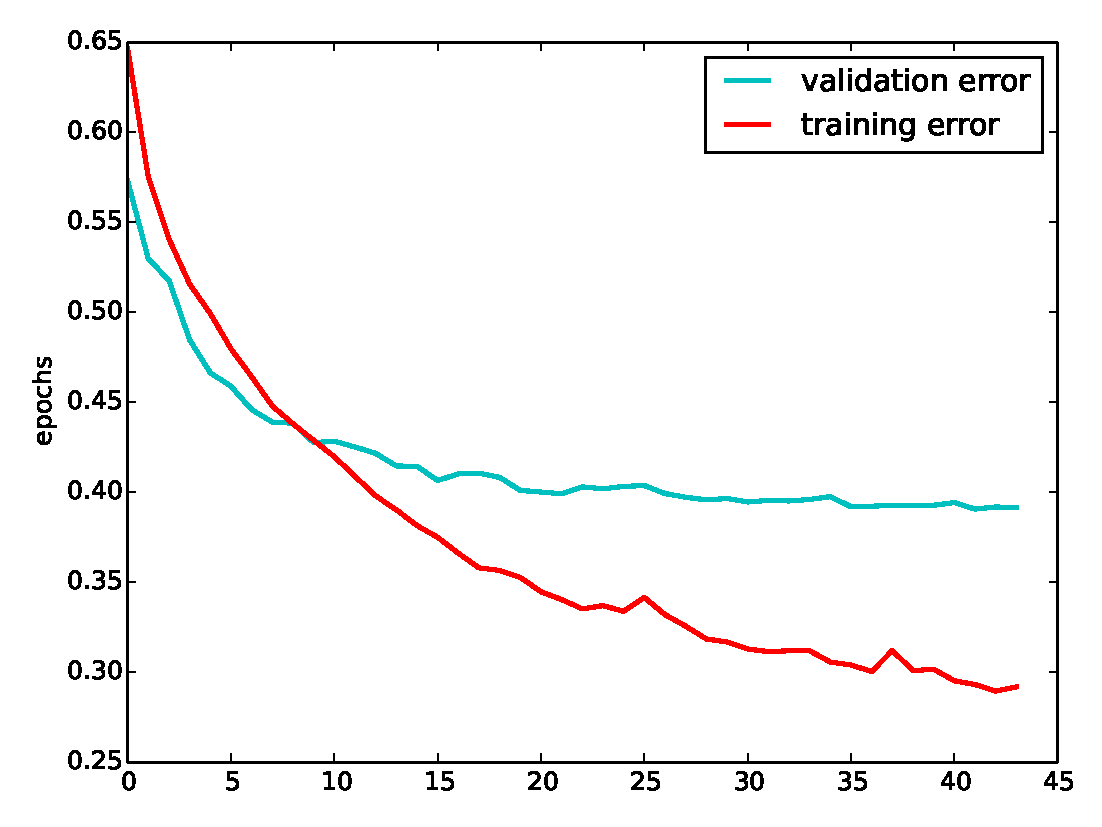
\includegraphics[width=.4\textwidth]{images/3dcnn_filters/training_error}
  \caption{The frame based error rate for training 3DCNN. The frame error rates from 3DCNN are much higher than the skeleton module in~\ref{sk_error_rate} which indicates learning from images may be more difficult than from skeleton modules. }\label{error rate}
\end{figure}

\subsubsection{Looking into the Networks: Visualisation of Filter Banks}

The convolutional filter weights of the first layer are depicted in Fig.~\ref{3dcnn_filters}. The unique characteristics from the kernels are clearly visible: For body and hand filters, both inputs are of the same size : $64\times64$. Hand inputs have larger homogenous areas than the body inputs, hence the hand part filters are smoother than the body part filters.

Depth images have sharper edges as also observed in~\cite{socher2012convolutional} and generally are smoother than the grayscale filters, though the distinctions are less obvious compared with the body versus hand filters.




\begin{figure}[t]
        \centering
        \begin{subfigure}[c]{.5\textwidth}
                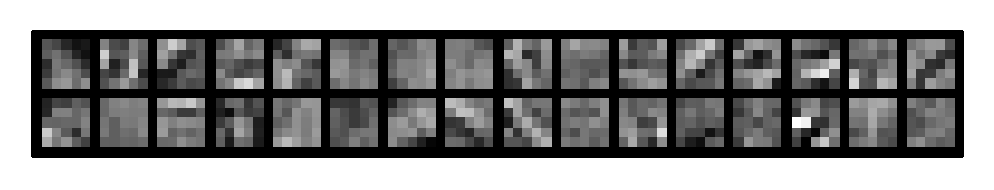
\includegraphics[width=\textwidth]{images/3dcnn_filters/gray_body_conv1_5_5}
                \caption{Grayscale body filters.}
                \label{Template_Image}
        \end{subfigure}%
        % ~ %add desired spacing between images, e. g. ~, \quad, \qquad, \hfill etc.
          %(or a blank line to force the subfigure onto a new line)

        \begin{subfigure}[c]{0.5\textwidth}
                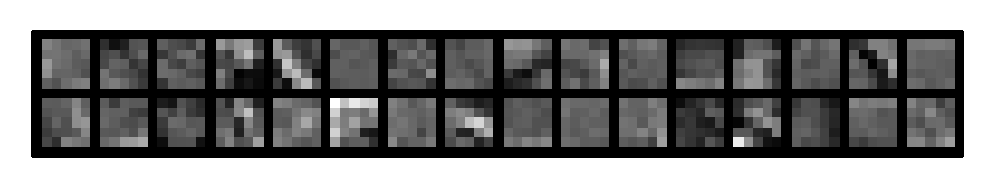
\includegraphics[width=\textwidth]{images/3dcnn_filters/depth_body_conv1_5_5}
                \caption{Depth body filters.}
                \label{Test_Image}
        \end{subfigure}

        \begin{subfigure}[c]{0.5\textwidth}
                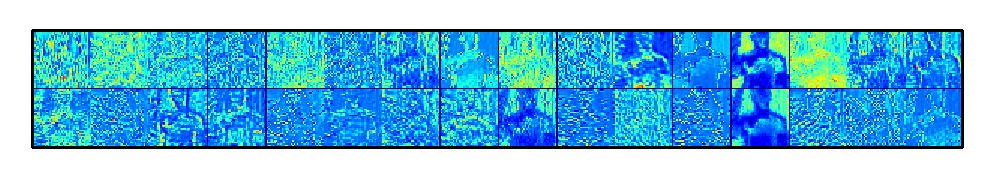
\includegraphics[width=\textwidth]{images/3dcnn_filters/filtered_images_body.eps}
                \caption{Response maps corresponds to body part.}
                \label{Test_Image}
        \end{subfigure}

        % ~ %add desired spacing between images, e. g. ~, \quad, \qquad, \hfill etc.
          %(or a blank line to force the subfigure onto a new line)
        \begin{subfigure}[c]{0.5\textwidth}
                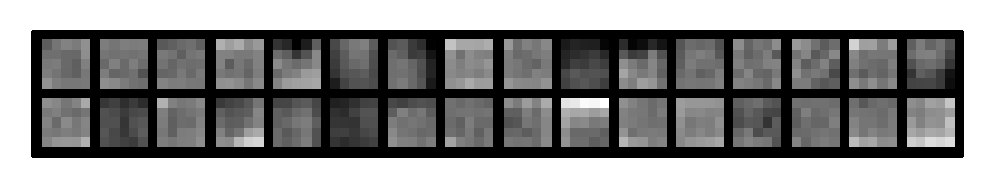
\includegraphics[width=\textwidth]{images/3dcnn_filters/gray_hand_conv1_5_5}
                \caption{Grayscale hand filters.}
                \label{Template_Response}
        \end{subfigure}

        \begin{subfigure}[c]{0.5\textwidth}
        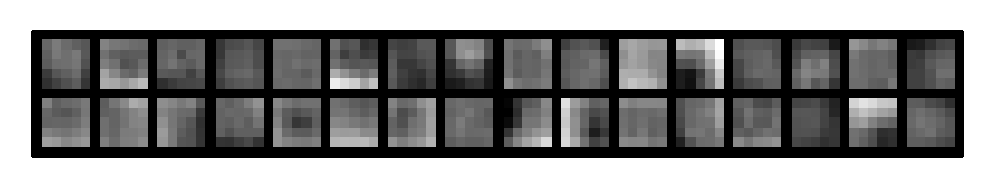
\includegraphics[width=\textwidth]{images/3dcnn_filters/depth_hand_conv1_5_5}
        \caption{Depth hand filters.}
        \label{shift-resize_image}
        \end{subfigure}

       \begin{subfigure}[c]{0.5\textwidth}
                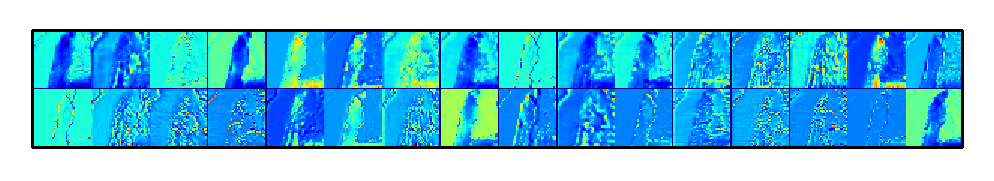
\includegraphics[width=\textwidth]{images/3dcnn_filters/filtered_images_hand.eps}
                \caption{Response maps corresponds to hand part.}
                \label{Test_Image}
        \end{subfigure}


        \caption{Visualisation of the $5\times5$ filters in the first layer for the different input channels. Interestingly, we observe the same effect as~\cite{socher2012convolutional} that the resulting filters from depth images have sharper edges which arise due to the strong discontinuities at object boundaries. While the depth channel is often quite noisy most of the features are still smooth. And response maps correspond to hand part are smoother than those correspond to body part.
        % Itcan be seen that the hand filters are smoother than the body part filters because hand input are smoother than the body part input.
        }\label{3dcnn_filters}
\end{figure}



%\begin{figure}[h]
%  \centering
%  % Requires \usepackage{graphicx}
%  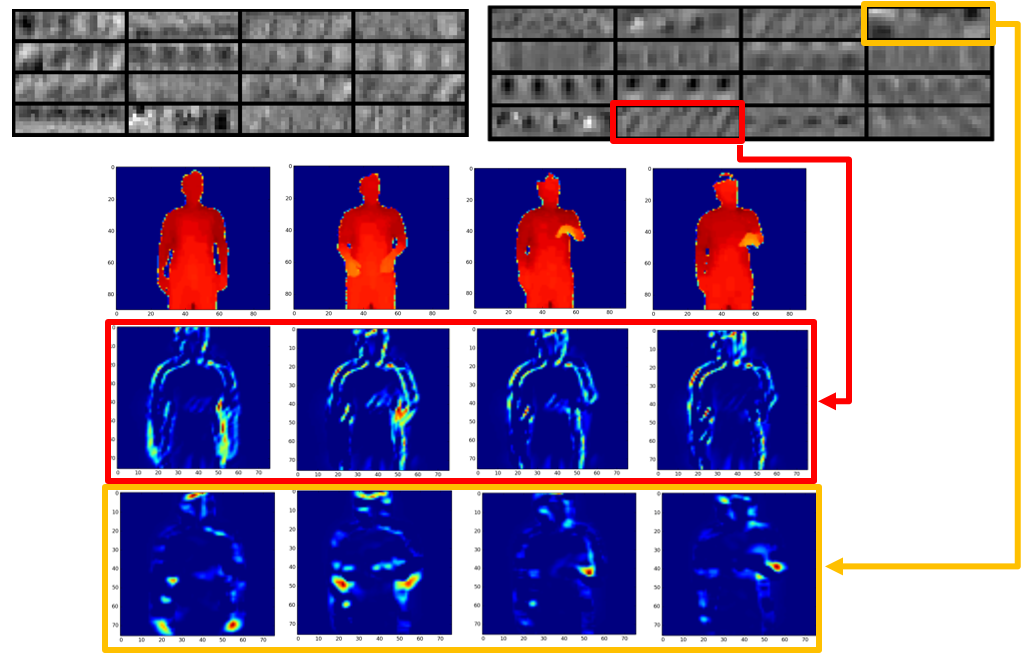
\includegraphics[width=0.5\textwidth]{images/filter_all_2}
%  \caption{{\footnotesize
%  Top left: the \emph{conv1} weights of the 3DCNN learnt with uncropped input; top right: the \emph{conv1} weights of the 3DCNN learnt with cropped input. It can be seen that filters/weights of the cropped input trained networks are smoother. Bottom: visualization of sample frames after \emph{conv1} layer (Sample0654, 264-296 frames, sampled every 8 frames). It can be seen that the filters of the first convolutional layer are able to learn both shape pattern(red bounding box) and motion(yellow bounding box). Also note that the high response maps correspond to the most informative part of the body, even though during the training process, all local patches are learned indiscriminately regardless of its location.}
%  }\label{conv1_vis}
%\end{figure}


%\begin{algorithm}[t]
%\caption{Normalization scheme 1: template matching}\label{normalization_scheme_1}
%\LinesNumbered
%\SetAlgoLined
%\SetAlgoNoEnd
%\DontPrintSemicolon
%\SetKwFunction{zeroes}{zeroes}
%\KwData{\;
%          $ \mathbf{T}$ - exemplary template with original scale of size $320 \times 320$,   \;
%           \hspace{0.5cm}   (Sample0003 is chosen as the exemplary template, shown in \ref{Template_Image}). \;
%          $ \mathbf{R_{depth}}$  - reference depth, fixed to $\textbf{\emph{1941}}$ (acquired from the above \;
%             \hspace{0.5cm} exemplary template  $ \mathbf{T}$). \;
%          $ \mathbf{\hat{T}}$ - test image, as shown in \ref{Test_Image}.\;
%          $ \mathbf{M}$ - user foreground segmented mask. \;
%            }
%        Apply a $5 \times 5$ aperture median filter to test depth frame $\mathbf{\hat{T}}$ as in~\cite{wu2012one} to reduce the salt and pepper noise. \;
%        Multiply test depth frame $\mathbf{\hat{T}}$ with the user segmented mask $ \mathbf{M}$: $\mathbf{\hat{T} = \hat{T} \times M}$. \;
%        Template matching test image $\mathbf{\hat{T}}$ with $ \mathbf{T}$ using normalized cross-correlation~\cite{lewis1995fast}, the response score $\mathbf{R}$  is shown in \ref{Template_Response}. \;
%        Shift the image according to the maximum response $\mathbf{R}$ to its centre applying affine transformation~\cite{opencv_library}. \;
%        Scale the image according to reference depth $ \mathbf{R_{depth}}$ and the median depth of a bounding box in the centre of the image with $25 \times 25$ size as shown as the green boundingp box in \ref{shift-resize_image}. \;
%        Resize the image from $320 \times 320$ to $90 \times 90$. \;
%
%
%\KwResult{\;
%        $ \mathbf{\tilde{T}}$ - Resize-normalized image shown in the yellow bounding box of \ref{shift-resize_image}.\;
%}
%\end{algorithm}
%\begin{algorithm}
%\caption{Normalization scheme 2: skeleton normalization}\label{normalization_scheme_2}
%\LinesNumbered
%\SetAlgoLined
%\SetAlgoNoEnd
%\DontPrintSemicolon
%\SetKwFunction{zeroes}{zeroes}
%\KwData{\;
%          $ \mathbf{S_{spine}}$ - Skeleton Spine joints pixel coordinates. \;
%          $ \mathbf{S_{shoulder}}$ - Skeleton Shoulder joints pixel coordinates. \;
%          $ \mathbf{\hat{T}}$ - test image.\;
%          $ \mathbf{M}$ - user foreground segmented mask. \;
%          $ \mathbf{R_{length}}$  - reference length of shoulder to spine, fixed to $\textbf{\emph{100}}$ (1 meter). \;
%            }
%        Apply a $5 \times 5$ aperture median filter to test depth frame $\mathbf{\hat{T}}$. \;
%        Multiply test depth frame $\mathbf{\hat{T}}$ with the user segmented mask $ \mathbf{M}$. \;
%        Shift the image according to the centroid of Spine joint $ \mathbf{S_{spine}}$.\;
%        Scale the image according to the $\mathbf{R_{length}}  / (\mathbf{S_{spine}} - \mathbf{S_{shoulder}})$. \;
%
%\KwResult{\;
%        $ \mathbf{\tilde{T}}$ - Resize the shifted-scaledp image to $90 \times 90$ .\;
%}
%\end{algorithm}
%\begin{figure}[t]
%        \centering
%        \begin{subfigure}[c]{0.2\textwidth}
%                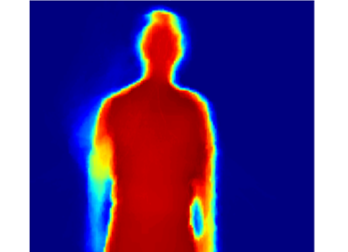
\includegraphics[width=\textwidth]{images/template3}
%                \caption{{\scriptsize template image}}
%                \label{Template_Image}
%        \end{subfigure}%
%        ~ %add desired spacing between images, e. g. ~, \quad, \qquad, \hfill etc.
%          %(or a blank line to force the subfigure onto a new line)
%        \begin{subfigure}[c]{0.2\textwidth}
%                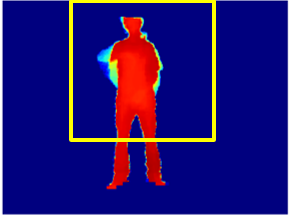
\includegraphics[width=\textwidth]{images/test1}
%                \caption{{\scriptsize test image}}
%                \label{Test_Image}
%        \end{subfigure}
%        ~ %add desired spacing between images, e. g. ~, \quad, \qquad, \hfill etc.
%          %(or a blank line to force the subfigure onto a new line)
%        \begin{subfigure}[c]{0.2\textwidth}
%                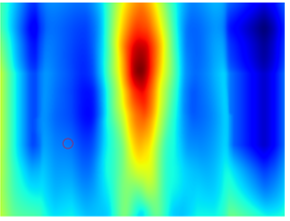
\includegraphics[width=\textwidth]{images/test3}
%                \caption{{\scriptsize template response}}
%                \label{Template_Response}
%        \end{subfigure}
%        \begin{subfigure}[c]{0.2\textwidth}
%        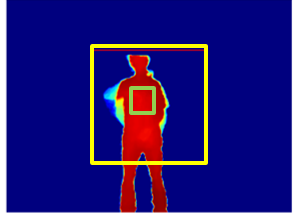
\includegraphics[width=\textwidth]{images/test2}
%        \caption{{\scriptsize shift-resize image}}
%        \label{shift-resize_image}
%        \end{subfigure}
%        \caption{{\footnotesize Illustration of normalization scheme 1: template matching.}}\label{Normalization scheme 1: template matching}
%\end{figure}

\subsection{Multimodal Fusion}

%\begin{figure}[t]
%  \centering
%  % Requires \usepackage{graphicx}
%  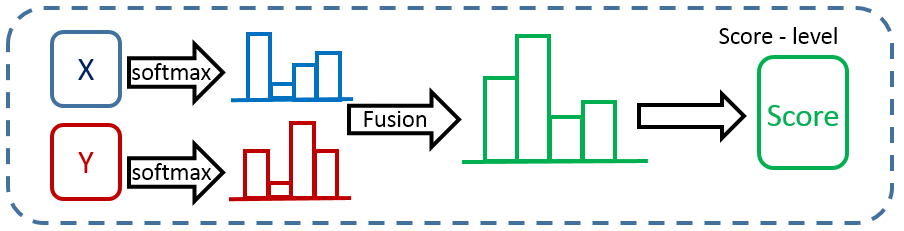
\includegraphics[width=0.45\textwidth]{images/fusion}
%  \caption{
% Illustration of late fusion. The coefficient is chosen using cross-validation using a validation set.
%  }\label{fusion}
%\end{figure}

\begin{figure}[t]
  \centering
  % Requires \usepackage{graphicx}
  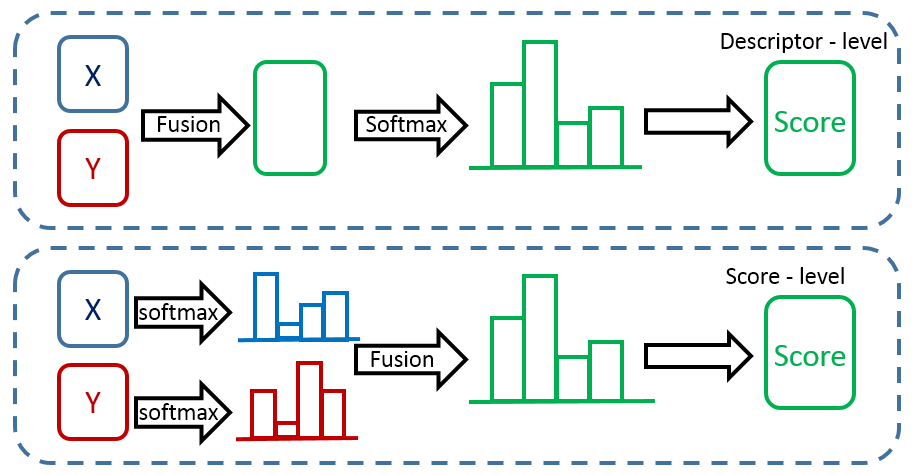
\includegraphics[width=0.45\textwidth]{images/Different_pipeline}
  \caption{{\footnotesize
        Different Pipelines for descriptor fusion.}
  }\label{fusion}
\end{figure}
To fuse both model predictions, the strategies shown in Fig.~\ref{fusion} are adopted.
\subsubsection{Late Fusion}




Formally, the multimodal fusion is a score fusion defined by:

\begin{equation}
 \mathbf{S} = \alpha*\mathbf{S^1} + (1-\alpha) * \mathbf{S^2}
\end{equation}
where $\mathbf{S^1}$ and $\mathbf{S^2}$ are the score probability matrices as in Algo.~\ref{MMDDN_test}, corresponding to the skeletal input and RGBD input, and $\alpha$ is the coefficient that controls the score balance obtained by cross validation.
Interestingly, the best performing $\alpha$ is close to $0.5$, thus indicating that both approaches perform comparably.

The complementary properties of both modules can be seen from the Viterbi path decoding plot in Fig.~\ref{Sample0700_comparison}.

\subsubsection{Early Fusion}\label{early_fusion}
\begin{figure*}[t]
  \centering
  % Requires \usepackage{graphicx}
  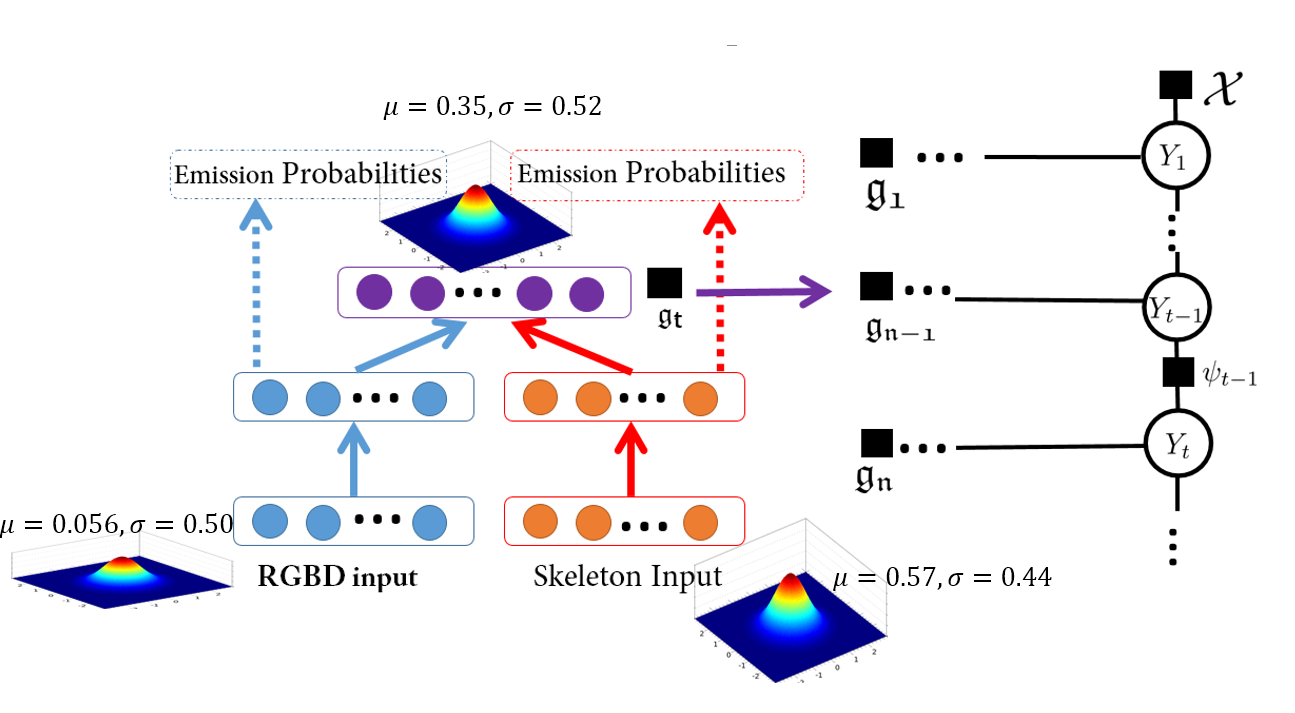
\includegraphics[width=0.75\textwidth]{images/early_fusion}
  \caption{
  Architecture of the multimodal dynamic networks: each modality (RGBD and skeleton) is first pre-trained by a Deep Neural Network, and their penultimate layers are fused together to generate a shared representation for dual modalities. The outputs are the emission probabilities $\mathfrak{g_t}$ for temporal dynamic modeling. The Gaussians represent activations of the neurons for each input modality and the final fusion layer. The mean activation of skeleton module neurons is predominantly larger than the RGBD ConvNet's (0.57 vs. 0.056). Note that skeleton module has logistic units whereas ConvNet module has leaky relu unit~\cite{DBLP:journals/corr/PigouODHD15}, hence the mean activations of the two are not directly comparable. However, 10 times the difference of mean activation indicates the bias during the multimodal fine-tuning phase that could cause the less than expected performance.
  }\label{early_fusion_fig}
\end{figure*}

Instead of traditional late fusion, we adopt another layer of perceptron(with 2024 hidden unites) for cross modality learning taking the input from each individual net's penultimate layer.
The parameters of two neural networks (for skeleton and depth) are loaded from the previously trained individual module. We argue that this ``pre-trained" parameters are important because the heterogenous inputs of the system.  We fine-tune the network and the stop the training when validation error rate stop decreasing ($\sim$15 epochs). The result for early fusion system are reported in Tab.~\ref{Table_score_fusion}.


However, we can see from Tab.~\ref{Table_score_fusion} that the early fusion system didn't outperform the late fusion system. The result is counter-intuitive because we expect the early fusion  multimodal feature learning will extract semantically meaningful shared representations, outperforming individual modalities, and the early fusion scheme�s efficacy against the traditional method of late fusion. One possible explanation could be that one individual module has dominant effect on the learning process so as to screw the network towards learning that specific module. The mean activations of the neurons for each modules in Fig.~\ref{early_fusion_fig} indicate the aforementioned conjecture.



\section{Experiments and Analysis}
\subsection{Chalearn LAP Data Set \& Evaluation Metrics} \label{sec:chalearn}
The data set\footnote{\href{http://gesture.chalearn.org/homewebsourcereferrals}{http://gesture.chalearn.org/homewebsourcereferrals}} used in this work is provided by the ChaLearn LAP \cite{chalearnLAP} gesture spotting challenge. The development set consists of 700 video sequences and 240 sequences are used for testing. The testing sequences however are not segmented a priori and the gestures must be detected within a continuous data stream. In total, there are more than $14\,000$ performed gestures.
% This dataset  is on ``multiple instance, user independent learning and continuous gesture spotting"~\cite{ICMI} of gestures.
% In the 3 track, there are more than 14,000 gestures.

For the input sequences, there are three modalities provided, \emph{i.e.} skeleton, RGB and depth images (with user segmentation). In the following experiments, the first 650 videos equences are used for training, 50 for validation and the other 240 for testing where each sequence contains around 10 to 20 gestures with some noisy non-meaningful vocabulary tokens.

The evaluation of this data set is performed using the Jaccard index, which computes the overlap between the ground truth and the predictions on a frame-by-frame basis:
\begin{equation}
J(A, B) = \frac{A \bigcap B}{A \bigcup B}
\end{equation}
where $A$ is the ground truth gesture label and $B$ is the predicted gesture label.


\begin{figure*}[t]
        \centering
        \begin{subfigure}[c]{.8\textwidth}
                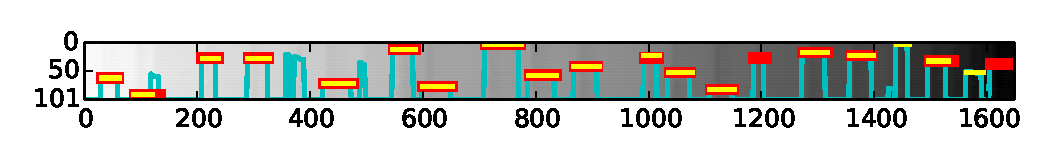
\includegraphics[width=\textwidth]{images/path/Sample0700_sk}
                \caption{Sample \#700 skeleton input path.}
                \label{Sample0700_sk}
        \end{subfigure}%
        ~ %add desired spacing between images, e. g. ~, \quad, \qquad, \hfill etc.
          %(or a blank line to force the subfigure onto a new line)

        \begin{subfigure}[c]{0.8\textwidth}
                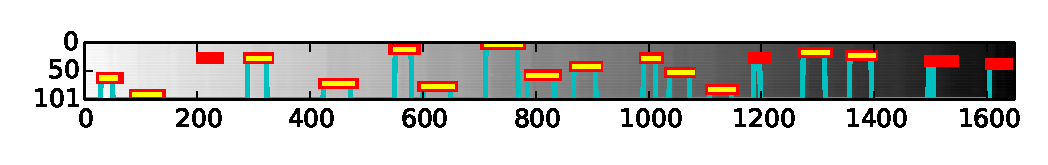
\includegraphics[width=\textwidth]{images/path/Sample0700_cnn}
                \caption{Sample \#700 depth and RGB input path.}
                \label{Sample0700_cnn}
        \end{subfigure}

        ~ %add desired spacing between images, e. g. ~, \quad, \qquad, \hfill etc.
          %(or a blank line to force the subfigure onto a new line)
        \begin{subfigure}[c]{0.8\textwidth}
                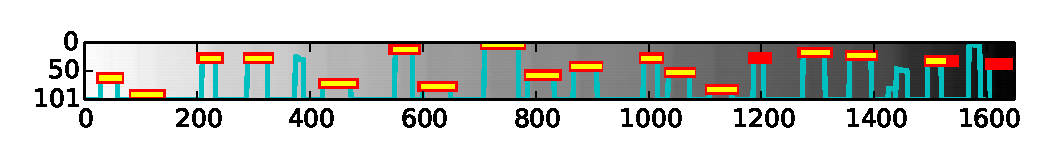
\includegraphics[width=\textwidth]{images/path/Sample0700_combined}
                \caption{Sample \#700 combined input path.}
                \label{Sample0700_combined}
        \end{subfigure}

  \caption{Viterbi decoding of the two modules and their fusion of sample sequence \#700. Top to bottom: skeleton, RGBD, multimodal fusion with x-axis representing the time and y-axis representing the hidden states of all the classes with the ergodic state at the bottom. Red lines are the ground truth labels, cyan lines represent the viterbi shortest path and yellow lines are the predicted labels. There are some complementary information of the two modules and generally the skeletal module outperforms the depth module. The fusion of the two could exploit the uncertainty, \emph{e.g.} around frame 200 the skeleton can help with the false negative predictions given by the 3DCNN module. Around frame 1450, the 3DCNN module can help suppress the false positive prediction given by skeleton module.
  }\label{Sample0700_comparison}
\end{figure*}

\subsection{Post-processing}
The predicted tokens that happen to be less than 20 frames are discarded as noisy tokens. Note that there are many noisy gesture tokens predicted by viterbi decoding. One way to sift through the noisy tokens is to discard the token path log probability smaller than a certain threshold. However, because we use the Jaccard index as evaluation score, it strongly penalises false negatives. Experiments show that the evaluation metric favours having more false positives than missing true positives. Effective ways to detect false positives should be an interesting aspect of future work.

\subsection{Results}

The individual module results and the fusion results are shown in Tab. \ref{Table_score_fusion}. Note that the skeleton module generally performs better than the depth module, one reason could be that the skeleton joints learnt from~\cite{shotton2011real} lie in success of utilising huge and highly varied training data: from both realistic and synthetic depth images, a total number of 1 million images were used to train the deep randomised decision forest classifier in order to avoid overfitting. Hence, skeleton data is more robust.

From the frame based prediction, we also evaluate the gesture token classification rate using the commonly-used PASCAL overlap criterion: if the gesture is predicted correctly with more than 50\% overlap with the ground truth label, then the prediction is counted as a true positive. The results of the two individual modules and the score of the fused modules are shown in Tab.~\ref{Prediction}. From the confusion matrices in Fig.~\ref{confusion_matrix} we can observe the complimentary information between the skeleton input and the RGBD input.
% with the confusion matrices shown in Fig.~\ref{confusion_matrix}.
While many of the gestures in this data set could be mainly differentiated by examining the positions and motions of large joints such as the elbows and wrists,  some gestures differ primarily  in hand pose, \emph{e.g.} Fig. \ref{hand_differ}.
% From the confusion matrices in Fig.~\ref{confusion_matrix} we can observe the complimentary information between the skeleton input and the depth \& RGB input.
%%%%%%%%%%%%%%%%%%%%%%%%%%%%%%%%%%%%%%%%%%%%%%%%%%%%%%%%%%
%%%%%%%%%%%%%%%%%%%%%%%%%%%%%%%%%%%%%%%%%%%%%%%%%%%%%%%%%%
 \begin{table}[t]
   \centering
        \begin{tabular}{|l||*{2}{c|}}\hline
            {Module}
            &\makebox[5em]{Validation}&\makebox[5em]{Test}
            \\\hline\hline
            {\small Skeleton -- DBDN }            &  0.78266    & 0.77920 \\\hline
            {\small RGBD -- 3DCNN }      &  0.75163    & 0.71678 \\\hline%\hline
            {\small Multimodal Late Fusion }              &  0.81744    & 0.80910 \\\hline
            {\small Multimodal Early Fusion }             &  0.80014    & 0.79800 \\\hline
        \end{tabular}

    \caption{
    Comparison of results in terms of Jaccard index between different network structures and various modules.
          }
          \label{Table_score_fusion}
\end{table}
%%%%%%%%%%%%%%%%%%%%%%%%%%%%%%%%%%%%%%%%%%%%%%%%%%%%%%%%%%


%%%%%%%%%%%%%%%%%%%%%%%%%%%%%%%%%%%%%%%%%%%%%%%%%%%%%%%%%%

 \begin{table}[rt]
   \centering
        \begin{tabular}{|ll||*{2}{c|}}\hline
            %\backslashbox{Module}{Evaluation Set}
             & &  \makebox[5em]{Validation}&\makebox[5em]{Test}       \\\hline\hline
            \multirow{2}{*}{Skeleton}       &{\small Acc}                & 0.8633     & 0.8360\\
                                            &  {\small UnRate}           & 0.0230     & 0.0412 \\\hline\hline
            \multirow{2}{*}{RGBD}    &{\small Acc }              & 0.7871     & 0.7581  \\
                                            &  {\small UnRate}           & 0.1612     & 0.1976 \\\hline\hline
            \multirow{2}{*}{Multimodal Late Fusion}   &{\small Acc }               & 0.8791     & 0.8642\\
                                            &  {\small UnRate}           & 0.0302     & 0.0485 \\\hline
           \multirow{2}{*}{Multimodal Early Fusion}   &{\small Acc }    & 0.8650     & 0.8545\\
                                            &  {\small UnRate}           & 0.0623     & 0.0768 \\\hline
        \end{tabular}

    \caption{
    Gesture classification accuracy (\emph{Acc}) and undetected rate (\emph{UnRate}): if the prediction overlaps with the ground truth with more than 50\%, it's considered a true positive.
          }
          \label{Prediction}
\end{table}

%%%%%%%%%%%%%%%%%%%%%%%%%%%%%%%%%%%%%%%%%%%%%%%%%%%%%%%%%%
%%%%%%%%%%%%%%%%%%%%%%%%%%%%%%%%%%%%%%%%%%%%%%%%%%%%%%%%%%
\begin{figure}[t]
        \centering
        \begin{subfigure}[c]{.36\textwidth}
                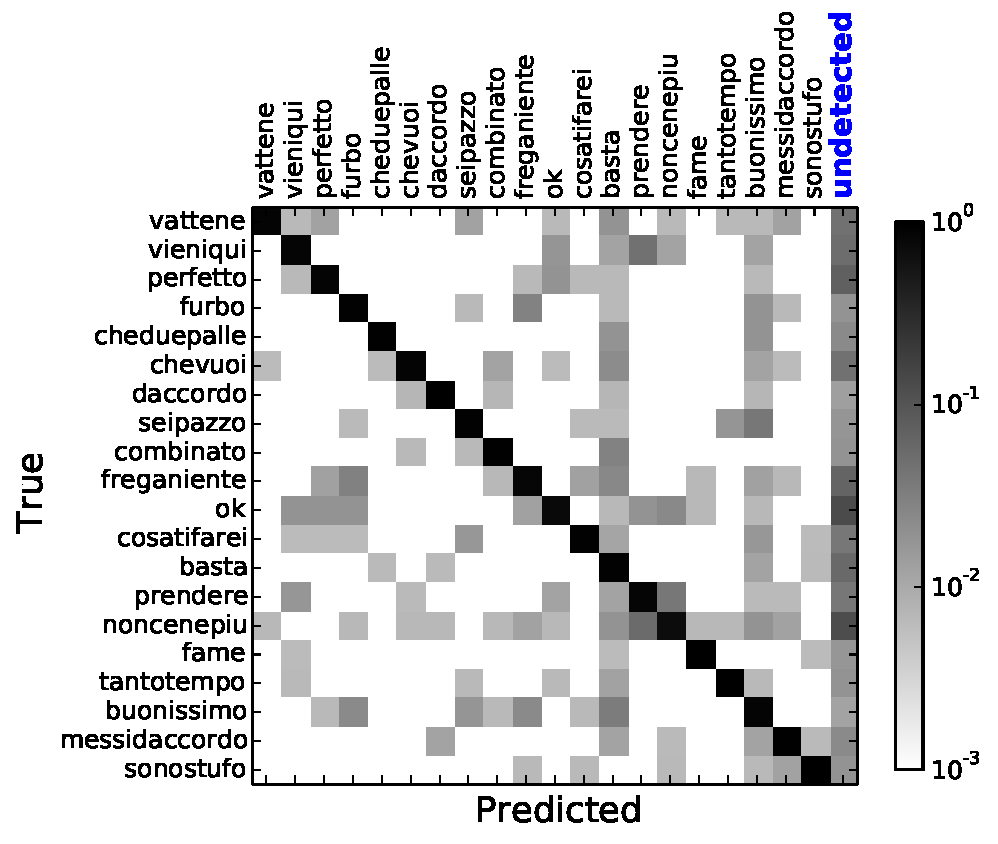
\includegraphics[width=\textwidth]{images/cm/cm_sk}
                \caption{Skeletal input prediction result.}
                \label{sk_cm}
        \end{subfigure}%
        ~ %add desired spacing between images, e. g. ~, \quad, \qquad, \hfill etc.
          %(or a blank line to force the subfigure onto a new line)

        \begin{subfigure}[c]{0.36\textwidth}
                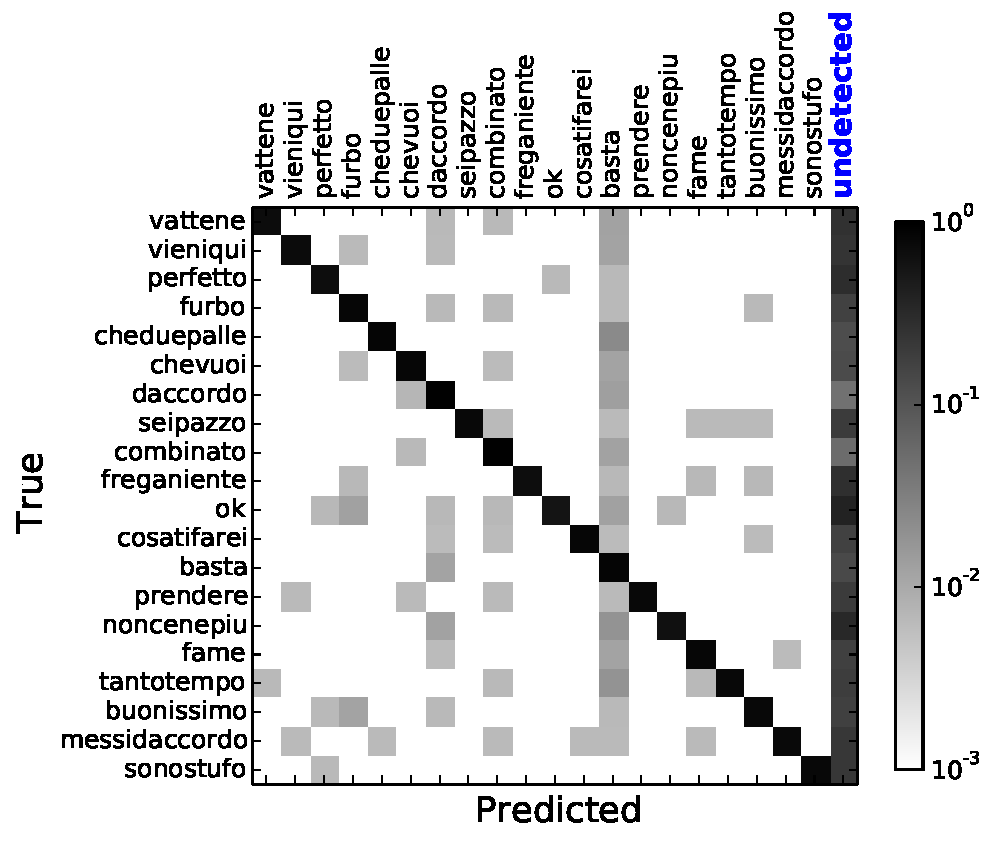
\includegraphics[width=\textwidth]{images/cm/cm_cnn}
                \caption{RGBD input prediction result.}
                \label{cnn_cm}
        \end{subfigure}

        ~ %add desired spacing between images, e. g. ~, \quad, \qquad, \hfill etc.
          %(or a blank line to force the subfigure onto a new line)
        \begin{subfigure}[c]{0.36\textwidth}
                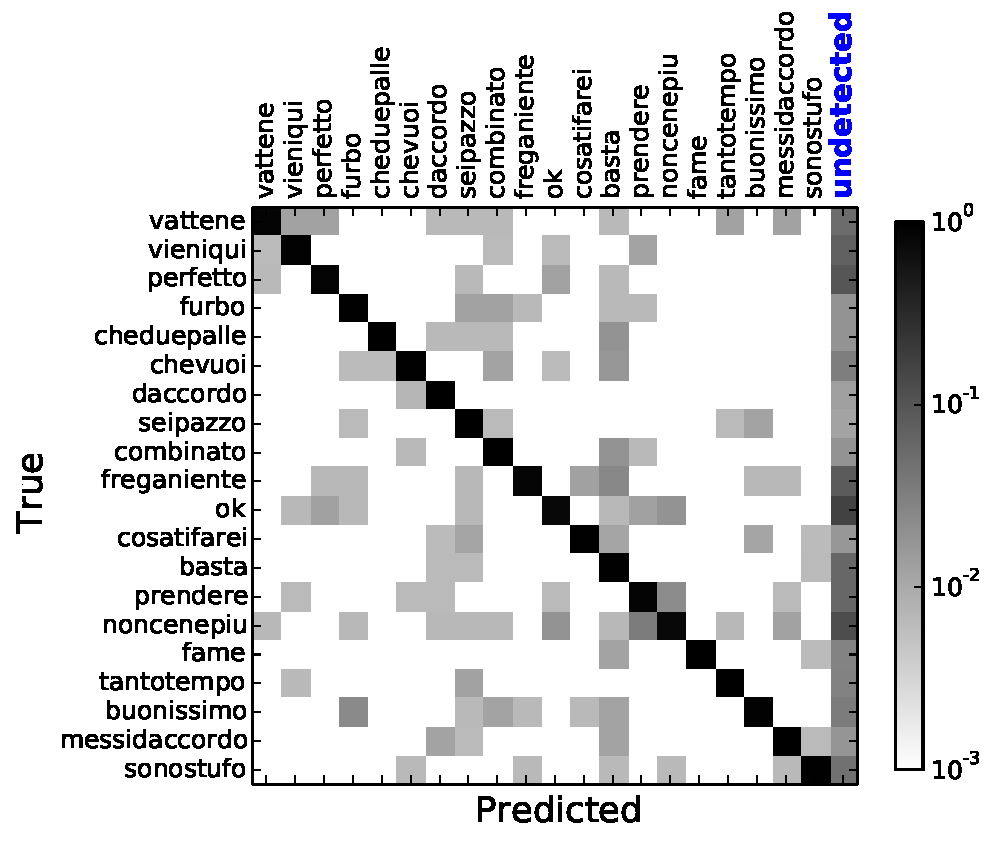
\includegraphics[width=\textwidth]{images/cm/cm_combination}
                \caption{Multimodal fusion prediction result.}
                \label{fusion_cm}
        \end{subfigure}

  \caption{Confusion Matrix for the skeletal input, RGBD input and multimodal fusion result.
  % Generally, the skeleton module has higher classification rate.
  Some gestures, \emph{e.g.} ``OK" and ``Non ce ne piu" differ primarily in hand poses. Hence, they are easier to be differentiated using the RGBD module than the skeleton module.
  }\label{confusion_matrix}
\end{figure}
%%%%%%%%%%%%%%%%%%%%%%%%%%%%%%%%%%%%%%%%%%%%%%%%%%%%%%%%%%

\begin{figure}[t]
        \centering


        \begin{subfigure}[c]{.2\textwidth}
        \centering
                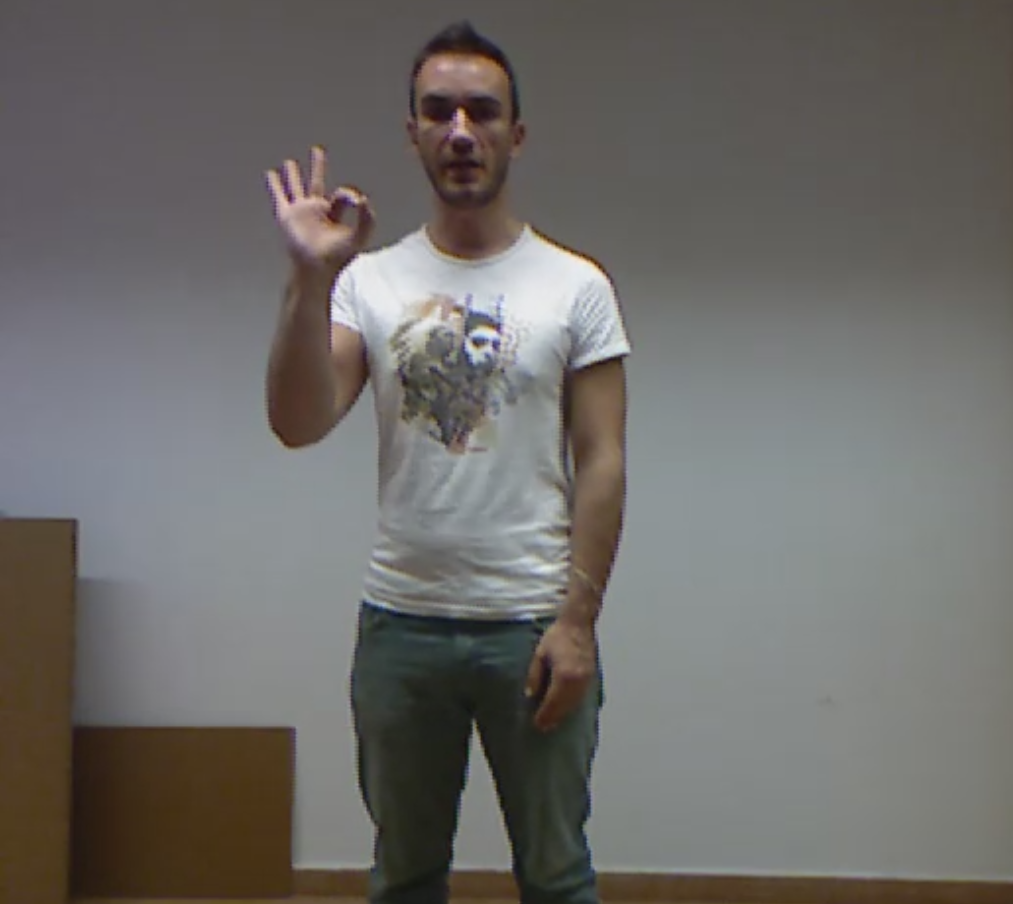
\includegraphics[width=3cm,height=3cm, trim=120 100 100 50, clip]{images/good}
                \caption{Well-recognised}
        \end{subfigure}%
        %
        \begin{subfigure}[c]{0.2\textwidth}
        \centering
                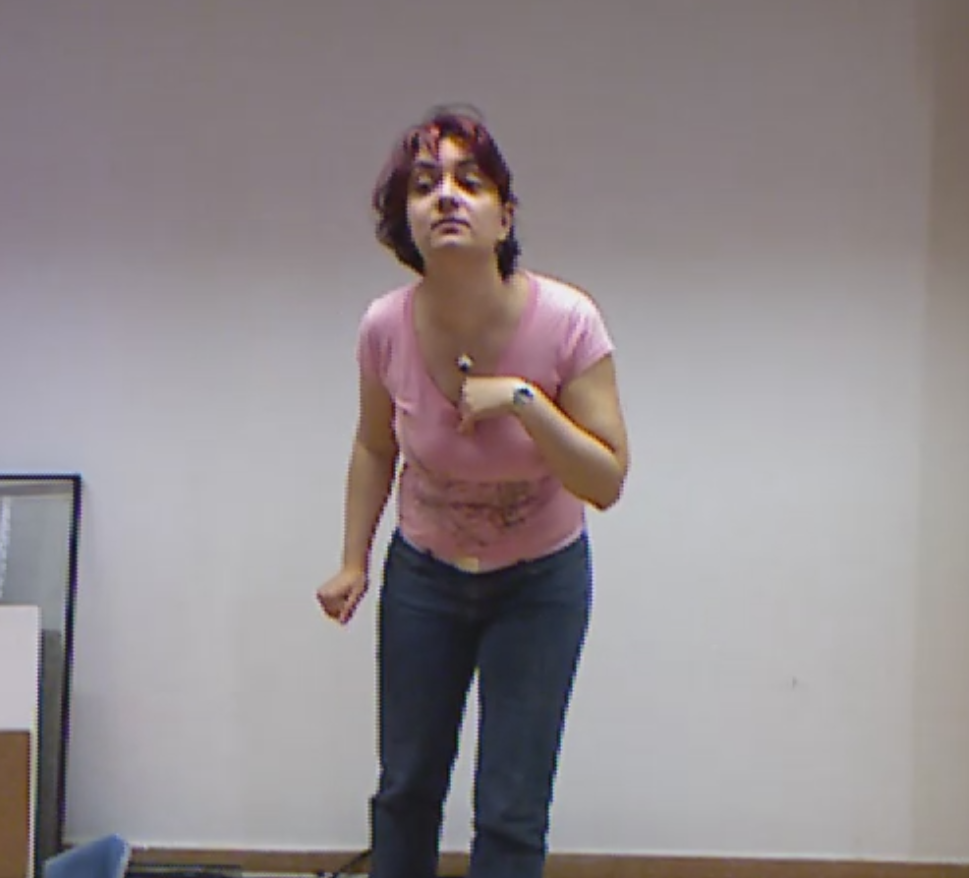
\includegraphics[width=3cm,height=3cm, trim=120 100 100 50, clip]{images/bad}
                \caption{Poorly-recognised}
        \end{subfigure}
  \caption{
  Examples of overall upper body movement's influence on system performance. Left (score: 0.94) performer almost kept static upper body whilst performing Italian sign language. Right (score: 0.34) performer moved vehemently when performing the gestures.
  }\label{good_bad_differ}
\end{figure}



\begin{figure}[t]
        \centering


        \begin{subfigure}[c]{.2\textwidth}
        \centering
                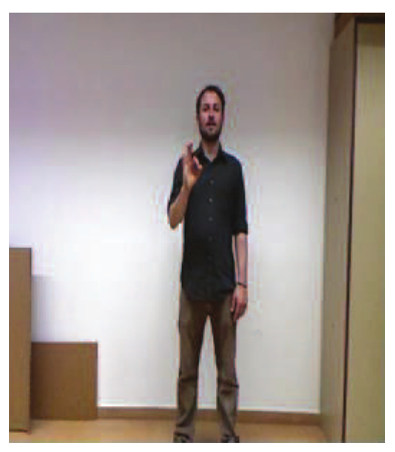
\includegraphics[width=2cm,height=3cm, trim=120 100 100 50, clip]{images/ok}
                \caption{``OK"}
        \end{subfigure}%
        %
        \begin{subfigure}[c]{0.2\textwidth}
        \centering
                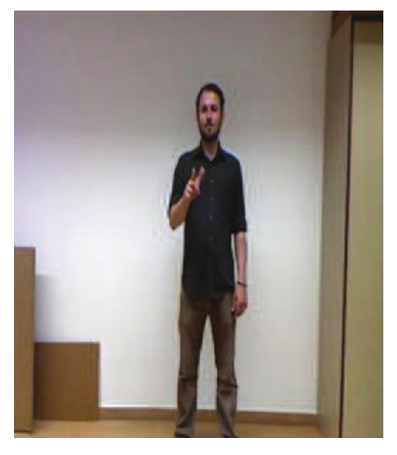
\includegraphics[width=2cm,height=3cm, trim=120 100 100 50, clip]{images/noncenepiu}
                \caption{``Non ce ne piu"}
        \end{subfigure}
  \caption{Examples of gestures that differ primarily in hand pose but not the arm motions.
  }\label{hand_differ}
\end{figure}

%%%%%%%%%%%%%%%%%%%%%%%%%%%%%%%%%%%%%%%%%%%%%%%%%%%%%%%%%%%%
 \begin{table}[t]
   \centering
        \begin{tabular}{|l||*{3}{c|}}\hline
            \backslashbox{Module}{Evaluation Set}
            &\makebox[3em]{Skeleton}&\makebox[6em]{RGBD}&\makebox[3em]{Fusion}
            \\\hline\hline
            {~\cite{neverova2014multi}} Deep Learning (Step 4)                  &   0.7891     &  0.7990      & \textbf{0.8449}\\\hline
            {~\cite{neverova2014multi}} Deep Learning (multiscal)               &   0.8080     &  0.8096      & \textbf{ 0.8488}\\\hline
            {~\cite{Monnier2014multi}} 3 Set Skeletal \& HOG                   &   0.791     & -           & 0.8220 \\\hline
            {~\cite{Chang2014multi}}   Handcrafted features                       &  \textbf{0.7948}     & -           & 0.8268\\\hline
            {~\cite{Peng2014multi}}    Dense Trajectory                         &  -          & \textbf{0.7919}      & -\\\hline
            {~\cite{lio2014deep}}      CNN                                      &  -          & 0.7888      & -\\\hline
            {~\cite{wu2014deep}}    Deep Learning                               &  0.7468     & 0.6371      & 0.8045\\\hline \hline
            \textbf{\emph{DDNN}} (this work)                                    &  0.7792    & 0.7168  & 0.8091\\\hline
        \end{tabular}
    \caption{
    Comparison of results in terms of Jaccard index between different network structures and various modules.
          }
          \label{Table_baseline}
\end{table}

\subsection{Computational Complexity}\label{Computational Complexity}
Although training the deep neural network using stochastic gradient descent is computationally intensive, once the model finishes training, our framework can perform real-time video sequence labelling with a low inference cost.
Specifically, a single feed forward neural network incurs linear computational time ($\mathcal{O}(T)$) and is efficient because it requires only matrix products and convolution operations. The complexity of the Viterbi algorithm is $\mathcal{O} (T* |S|^2)$ with $T$ the number of frames and $|S|$ the number of states.

Using a modern GPU (GeForece GTX TITAN Black), our multimodal neural network can be deployed at 90 FPS using Theano library~\cite{Bastien-Theano-2012} which is 6 times of real time (15 FPS). The preprocessing part takes most of the time and our un-optimized preprocessing pipeline is 25 FPS and Viterbi decoding is 90 FPS. Hence, the overall system can achieve faster than real-time performance.

\section{Conclusion and Discussion}

Hand-engineered, task-specific features are often less adaptive and time-consuming to design. This difficulty is more pronounced with multimodal data as the features have to relate with multiple data sources.
In this paper, we presented a novel deep dynamic neural network (DDNN) framework that utilises deep belief betworks and 3D convolutional neural networks for learning contextual frame-level representations and modelling emission probabilities for Markov fields.
 The heterogeneous inputs from skeletal joints, RGB and depth images require different feature learning methods and the late fusion scheme is adopted at the score level. The experimental results on bi-modal time series data show that the multimodal DDNN framework can learn a good model of the joint space of multiple sensory inputs, and is consistently as good as or better than the unimodal input, opening the door for exploring the complementary representation among multimodal inputs. It also suggests that learning features directly from data is a very important research direction and with more and more data and flops-free  computational power, the learning-based methods are not only more generalisable to many domains, but also are powerful in combining with other well-studied probabilistic graphical models for modelling and reasoning dynamic sequences.
Future works include learning the share representation amongst the heterogeneous inputs at the penultimate layer and backpropagating the gradient in the share space in a unified representation.


\appendices
% you can choose not to have a title for an appendix
% if you want by leaving the argument blank
\section{Details of the Code}
The python code for this work can be found at: \\
\footnotesize{\verb+https://github.com/stevenwudi/chalearn2014_wudi_lio+}


% use section* for acknowledgment
\ifCLASSOPTIONcompsoc
  % The Computer Society usually uses the plural form
  \section*{Acknowledgments}
\else
  % regular IEEE prefers the singular form
  \section*{Acknowledgment}
\fi

The authors would like to thank Sander Dieleman for his guidance in building, training and initialising convolutional neural networks.


\bibliographystyle{IEEEtran}
\bibliography{tPAMI2015}

\newpage

\newpage

\section{Review}

\subsection{Editor Comments}
Associate Editor
Comments to the Author:
Reviews of the paper have been received. In general comments are positive. Still one reviewer suggests some interesting extra analyses of the proposed method. Please carefully address all reviewers comments for a second review round of the paper. Please provide your revision by July 31th.


\hfill

\textbf{Response:}
We�d like to thank the associate editor's general positive comments on our paper. We also would like to thank reviewers' careful and insightful suggestions for improving the paper. Following are some common points that were mentioned by the reviewers and we list the most notable changes below. The point to point responses are provided afterwards.



\begin{itemize}
\item In the previous version for multimodal fusion, we used the late fusion scheme  $s = a * s1 + (1-a)*s2$ where $a$ is chosen by cross-validation. In this revision, we implement an early fusion scheme in Section~\ref{early_fusion} that a new-top level perceptron layer is created to combine two models' output as in Fig.~\ref{early_fusion_fig}. The new multimodal neural network's parameters are initialised by the previously trained individual module, taking advantage of different modules� intrinsic properties and making the network converge much faster. The early fusion system uses pre-trained weights. The results are reported in  Section~\ref{early_fusion} and Table~\ref{Table_score_fusion}.

\item The Related Works section has been moved after the Introduction section. We also follow reviewers' suggestions and include discussions of related works concerning works of: 1) exploiting temporal models in the context of gesture recognition; 2) literature for RGBD data using deep learning -
    ``Wang \emph{et al.}~\cite{wang2006hidden} introduced a discriminative hidden-state approach for the recognition of human gestures. However, their discriminative training is limited for pre-segmented gesture sequences and one layer of hidden states might not learn powerful enough high level representations for a larger corpus."
    ``In the field of deep learning from RGBD data, Socher \emph{et al.}~\cite{socher2012convolutional} proposed a single convolutional neural net layer for each modality as input to multiple, fixed-tree RNNs in order to compose higher order features for 3D object classification. The single convolutional neural net layer provides useful translational invariance of low level features such as edges and allows parts of an object to be deformable to some extent. The pooled filter responses are then given to a recursive neural network to learn compositional features and part interactions.
    Gupta \emph{et al.}~\cite{gupta2014learning} proposed a geocentric embedding for depth images that encodes height above ground and angle with gravity for each pixel in addition to the horizontal disparity. The depth image was represented by three channels: horizontal disparity, height above ground and angle with gravity. This augmented representation allows the CNN to learn strong features than by using disparity (or depth) alone. "

\item Experimental analysis. We have included some time analysis in Section~\ref{Computational Complexity} and visualisation of response maps after learnt filters in Fig~\ref{3dcnn_filters}.

\item Explanation of intuition behind higher level presentation of the skeleton features. We include Section \ref{Deep Dynamic Neural Networks} to explain the intuition behind higher level representation for skeleton joint features which appeared in our previous CVPR paper but was not included in the previous submission. We think this part is one of major contributions of the paper and inclusion of this section makes the journal paper more self-contained.
\end{itemize}

\hrulefill

\subsection{Reviewer Comments}
\subsubsection{Reviewer1}
\emph{Recommendation: Accept With No Changes}

\emph{\textbf{Comments:} The article is easy to read and well structured. The methodology is not strictly novel but its application in the gesture domain with the multimodal fusion makes the article worth reading. Although results are arguably a little behind the maximum performance ones the overall impression of the article is favorable and I believe the community may benefit to check the ideas included in this paper. }

\emph{ The article proposes a framework for dynamic data augmenting a HMM with deep learning techniques and apply this to gesture segmentation and recognition. Gestures segmentation and recognition is a difficult problem. The article tackles this difficulty by means of pure data driven approaches similar to the ones used for speech recognition. The particularities of the computer vision domain are handled accordingly.}

\textbf{Response:} Thank you for your review and positive outlook of the paper. We are also aware that our results are arguably a little behind the maximum performance, and this may be due to the network initialisation and multimodal neural network learning. We have included extra experimental analysis and early fusion implementation to further extend the broadness of the paper.

\hrulefill

\subsubsection{Reviewer2}
\emph{Recommendation: Revise and resubmit as �new�}

\textbf{\emph{Comments:}}
\emph{In general, the manuscript is well written and is easy to follow. In the given case, it would be preferable to have the "Related work" section right after the introduction, as otherwise paper's contributions are not completely clear. Furthermore, there is certainly a vast literature on exploiting HMMs in the context of gesture recognition (as well as other temporal models, such as recurrent neural networks), which should be briefly summarized, the differences with the proposed solution should be highlighted.}

\textbf{Response:}
Thank you for your comments and the recognition of easy readability of the paper. We have moved the related work section after the introduction section. Moreover, we have included the discussions of literature that utilise temporal models, e.g.,``Wang \emph{et al.}~\cite{wang2006hidden} introduced a discriminative hidden-state approach for the recognition of human gestures. However, their discriminative training is limited for pre-segmented gesture sequences and one layer of hidden states might not learn powerful enough high level representations for a larger corpus",  ``~\cite{socher2012convolutional} proposed a single convolutional neural net layer for each modality as input to multiple, fixed-tree RNNs in order to compose higher order features for 3D object classification."


\hfill

\textbf{\emph{Comments:}}
\emph{Authors claim to learn a model in the joint multi-modal space is a slight overstatement, as neural networks processing different modalities are trained completely independently with following averaging of produced scores.}

\textbf{Response:}
Thank you for your comments. In this revision, we implement the early fusion scheme in Section~\ref{early_fusion} that ``we adopt another layer of perceptron for cross modality learning taking the input from each individual net's penultimate layer.
The parameters of two neural networks (for skeleton and depth) are loaded from the previously trained individual module...The results for the early fusion system are reported in Tab.~\ref{Table_score_fusion}. The fusion network is initialised by the pre-trained model and stacked with one hidden layer with 2024 hidden unites. We fine-tune the network and stop the training when the validation error rate stops decreasing ($\sim$15 epochs)...However, we can see from Tab.~\ref{Table_score_fusion} that the early fusion system does not outperform the late fusion system. The result is counter-intuitive because we expect that the early fusion  multimodal feature learning would extract semantically meaningful shared representations, outperforming individual modalities, and the early fusion scheme�s efficacy against the traditional method of late fusion~\cite{wu2014multimodal}. One possible explanation could be that one individual module has dominant effect on the learning process so as to screw the network towards learning that specific module. The mean activations of the neurons for each module in Fig.~\ref{early_fusion_fig} indicate the aforementioned conjecture."

\hfill

\textbf{\emph{Comments:}}
\emph{State of the art in the experimental section should be mentioned more consistently. For fair comparison, first three lines in Table 3 should be:
[39] Deep learning (step 4): skeleton 0.7891, video 0.7990, fusion 0.8449 [39] Deep learning (multiscale): skeleton 0.8080, video 0.8096, fusion 0.8488 [40] 3 sets of skeletal features and HoG: skeleton 0.791, fusion 0.8220
Therefore, it shows that both learning-based and feature extraction-based approaches outperform the proposed method on each modality, as well as on a combination of them.
Furthermore, it would be interesting to see how the HMM contributes in the performance in comparison with simple voting based on frame-based predictions.}

\textbf{Response:}
Thank you for your detailed comments. We have amended the results table accordingly. The less than maximum performance could be due to the less than ideal settings and initialisations of the neural network. Nonetheless, we would like to argue that one major contribution of the paper is using the learning method for feature extraction and the utilisation of HMM for simultaneous gesture segmentation and recognition. We also present some brief analysis of why the fusion network didn't achieve expected performance gain and hope the experimental analysis could cast some light on the future research directions of the related problems.

\hfill

\textbf{\emph{Comments:}}
\emph{Visualization of the filter banks (section 3.3.4) in its current state is unnecessary as it does not provide any interesting insights on the interpretation of the learned features. Instead, the poorly formed filters rather indicate undertraining, or lack of training data given the model complexity, or suboptimality of training procedure.}

\textbf{Response:} We  include the response maps after filtering for both body and hand parts. We observe some interesting properties from the visualisation of the filter banks as in~\cite{socher2012convolutional} that ``Depth images have sharper edges and generally are smoother than the grayscale filters, though the distinctions are less obvious compared with the body versus hand filters."




\hrulefill

\subsubsection{Reviewer3}
\emph{Recommendation: Author Should Prepare A Minor Revision}

\textbf{\emph{Comments:}}

\emph{In general, I would be more excited if shared representations were learned from the skeleton and the RGB data, as done in multimodal deep learning. This is left for future work.  On the positive side, the CNN and DBN are technically sound and the results from their fusion are interesting.}

\emph{One would expect that the journal version of the paper would be more self-contained and easier to follow than the conference versions, but here I observe the opposite trend. For example, the older conference version ~\cite{diwucvpr14} explains the intuition behind the higher level representation of the skeleton features, but the journal version does not. The conference paper explains how the coordinate frames are built for the features, while this paper skips this part. The conference paper explains the datasets and visualizes the Viterbi paths better.}

\textbf{Response:} Thank you for your careful and positive review. We agree that in this journal version of the paper, some self-contained information has been omitted from the conference paper. In this revision, we have included more details. Specifically, 1) we include the Problem formation in Sec~\ref{Problem formation} that explains the intuition behind the higher level representation and the advantages offered by feed forward neural over GMMs. 2) we include another section for learning the higher level representation for skeleton joints features in Section~\ref{skeleon_high_level} from a pre-training point of view. The pre-training step is of crucial importance in learning the right initialisation of the deep belief networks using the sigmoid activation function.


\hfill

\textbf{\emph{Comments:}}
\emph{Section 2 does not help much the reader understand the formulation. For example:
 "At each time step, we have one observed random variable $X_t$: explain what these variables represent early (raw skeletan input / RGBD)  we have an unobserved variable $H_t$: describe at a high level the information that the unobserved variables capture, mention examples}

\textbf{Response:}
We have included the interpretation part as follows: ``A continuous-observation HMM with discrete hidden states is adopted for modelling higher level temporal relationships. At each time step $t$, we have one observed random variable $X_t$ which can be the skeleton input or depth/RGB input.
 The unobserved variable $H_t$ taking on values in a finite set  $\mathcal{H}=(\bigcup _{a \in \mathcal{A}} \mathcal{H}_a)$, where $\mathcal{H}_a$ is a set of states associated with an individual gesture $\textbf{\emph{a}}$ by force-alignment. The unobserved variable $H_t$ can be interpreted as a segment of an action $\textbf{\emph{a}}$. For example, for action sequence ``tennis serving", the action sequence can be dissected into $\mathcal{H}_{a_1}, \mathcal{H}_{a_2}, \mathcal{H}_{a_3}$ as: 1) raising one arm, 2) raising the racket, and 3) hitting the ball."



\hfill

\textbf{\emph{Comments:}}
\emph{The related work section is out of place after the technical sections and before the experiments.}

\textbf{Response:} We have moved the related work section after the introduction section.


\hfill

\textbf{\emph{Comments:}}
\emph{There is no point writing a loop for m=1:2 in Algorithm 1 and 2.}

\textbf{Response:} We have rewritten Algorithms 1 and 2 and merge the algorithms into a more succinct format.

\hfill

\textbf{\emph{Comments:}}
\emph{"the number of states ... is chosen as 5": any intuition here?}

\textbf{Response:} Thank you for the comment and this is a very good observation. The number of hidden states chosen uniformly as 5 in the paper might not be the optimal way of setting the number of hidden states for each gesture. We also experimented segmenting gestures into 10 states and obtained similar results. We reduce the hidden states from 10 to 5 in order to reduce the number of predicting classes and avoiding overfitting. The interpretation of choosing the number of hidden states for Markove Model is similar to choosing the number of hidden states for neural networks: it's more heuristically based. Ideally, we could set the number of hidden states according to the average length of the gesture sequence. But due to time constraint, we didn't train such neural networks.

\hfill

\textbf{\emph{Comments:}}
\emph{"10 frames are assigned to hidden state ...": why 10?}

\textbf{Response:} Thank you for the careful observation. This is actually a written error due to different number of hidden states used for our experiments. We rewrote the section as:
``\textbf{\emph{Hidden states} ($\mathcal{H}_a$): } Force alignment is used to extract the hidden states, \emph{i.e.} if a gesture token is 100 frames, the first $20= \frac{100}{5(N_{\mathcal{H}_a} )}$ frames are assigned to hidden state $\textbf{\emph{1}}$, the following 20 frames are assigned to hidden state $\textbf{\emph{2}}$, and so forth."



\hfill

\textbf{\emph{Comments:}}
\emph{it is hard to interpret the learned features on Figure 8. There is no intuition what the depth filters capture.}

\textbf{Response:} Because our filter size is $5\times5$ (smaller filter sizes tend to generalize better, ~\cite{simonyan2014very} used $3\times3$ convolution filters), it will be hard to interpret. However, we observe the similar effect as in paper~\cite{socher2012convolutional} for depth image filters and we include the following analysis:
``Visualisation of the $5\times5$ filters in the first layer for the different input channels . Interestingly, we observe the same effect as~\cite{socher2012convolutional} that the resulting filters from depth images have sharper edges which arise due to the strong discontinuities at object boundaries. While the depth channel is often quite noisy, most of the features are still smooth."

\hfill

%\textbf{\emph{Comments:}}
%\emph{ "multiple channel fusion outperforms individual modules by a large margin.": the difference is rather small based on the experiments}
%
%\textbf{Response:}


\hfill

\textbf{\emph{Comments:}}
\emph{Citations that could be added in the context of deep learning from RGBD data: "Convolutional-Recursive Deep Learning for 3D Object Classification", Socher et al., NIPS 2012}

\textbf{Response:}
Thank you for the suggested citation. And we now include in the related works section as follows:``In the field of deep learning from RGBD data, Socher \emph{et al.}~\cite{socher2012convolutional} proposed a single convolutional neural net layer for each modality as input to multiple, fixed-tree RNNs in order to compose higher order features for 3D object classification. The single convolutional neural net layer provides useful translational invariance of low level features such as edges and allows parts of an object to be deformable to some extent. The pooled filter responses are then given to a recursive neural network to learn compositional features and part interactions."

We also observe the same CNN filters as the paper that ``one interesting result is that depth channel edges are much sharper. This is due to the large discontinuities between object boundaries and background. While the depth channel is often quite noisy, most of the features are still smooth".

\hfill

\textbf{\emph{Comments:}}
\emph{"Learning Rich Features from RGB-D Images for Object Detection and Segmentation", Gupta et al., ECCV 2014}

\textbf{Response:}
We find the works in Gupta \emph{et al.}~\cite{gupta2014learning} interesting in a sense that CNN does not necessarily need to be trained from the raw images, and some handcrafted features may better help the network to learn more meaningful, higher level representations. And we have included this related work as follows.
``Gupta \emph{et al.} proposed a geocentric embedding for depth images that encodes height above ground and angle with gravity for each pixel in addition to the horizontal disparity. The depth image was represented by three channels: horizontal disparity, height above ground and angle with gravity. This augmented representation allows the CNN to learn strong features than by using disparity (or depth) alone."

\hfill

\textbf{\emph{Comments:}}
\emph{Another related work is the "Multimodal Deep Learning" by Ngiam et al., ICML 11. I would also like to see some discussion wrt "Hidden Conditional Random Fields for Gesture Recognition", Wang et al, CVPR 2006}

\textbf{Response:}
Thank you for suggesting very relevant works. We came across both papers. "Multimodal Deep Learning" essentially is the prototype for an early fusion model. Wang \emph{et al.}~\cite{wang2006hidden}) observed that one hidden layer is limited for learning a larger class corpus. Feature learning for skeleton modules is an essential part of this paper and we believe a higher level representation is more beneficial for gesture classification. Moreover, the partition function of CRF makes the discriminative training more difficult to train.  The similarity in the aforementioned paper with our proposed method is that both methods used a hidden layer for learning higher level representations. Recent advancement in feature learning and pre-training for DBN renders our proposed method more meaningful. We have included the following in the related works section:
``Wang \emph{et al.}~\cite{wang2006hidden} introduced a discriminative hidden-state approach for the recognition of human gestures. However, their discriminative training is limited for pre-segmented gesture sequences and one layer of hidden states might not learn powerful enough high level representation for a larger corpus."

\hfill

\hrulefill
\subsubsection{Reviewer4}
\emph{Recommendation: Author Should Prepare A Major Revision For A Second Review}

\textbf{\emph{Comments:}}
\emph{Late fusion: my greatest technical concern is that two deep models are trained and then combined with a weighted average: s = a * s1 + (1-a)*s2 where a is chosen by cross-validation. Instead, the authors could combine the two models by creating a new top-level perceptron layer which takes the two models as input. Then this whole structure could be trained jointly with back-propagation. I'd expect results to be (1)at least as good and (2) more philosophically unified. }

\textbf{Response:} We agree with your insightful observation and continue experimenting with the early fusion scheme in this revision. Our previous paper~\cite{wu2014multimodal} utilized the early fusion scheme for audio and skeleton modules for action recognition. We followed that strategy and perform the early fusion scheme using penultimate layer in Section\ref{early_fusion}.
``However, we can see from Table~\ref{Table_score_fusion} that the early fusion system does not outperform the late fusion system. The result is counter-intuitive because we expect that the early fusion  multimodal feature learning would extract semantically meaningful shared representations, outperforming individual modalities, and the early fusion scheme�s efficacy against the traditional method of late fusion~\cite{wu2014multimodal}. One possible explanation could be that one individual module has the dominant effect on the learning process so as to screw the network towards learning that specific module. The mean activations of the neurons for each modules in Fig.~\ref{early_fusion_fig} indicate the aforementioned conjecture."

\hfill

\textbf{\emph{Comments:}}
\emph{The analysis is a bit brief. More experiments and ablative analysis could be added. Specifically, can we interpret the failure patterns of the proposed model(s) and prior work? It would be interesting to see statements like [40] fails more often on gestures of X kind because HOG erases Y useful information or [39] does worse for Z because it handles time at an earlier stage of the pipeline. Then, also giving some qualitative examples of these failures.}

\textbf{Response:}
We agree that there is a lack of experiments� analysis, especially the failure patterns and lessons learnt from the experiments. We have included more analysis in the Experiment and Analysis section as follows:
``Examples of overall upper body movements� influence on the system performance. Left (score: 0.94) performer almost kept a static upper body whilst performing Italian sign language. Right (score: 0.34) performer moved vehemently when performing the gestures.\ref{good_bad_differ}"


\hfill

\textbf{\emph{Comments:}}
\emph{These extra experiments (considering joint training of a combined emission probability model) and qualitative interpretation could significantly affect the paper. Overall, the research is solid but needs significantly more work before publication.
RCNN: Last, it is entirely possible to train a recurrent neural network to perform Viterbi decoding. This may be difficult (requiring more training data) but would make the entire paper fit into a the deep learning framework. I cannot hold this against the authors, but some discussion might help.}

\textbf{Response:}
We have included more qualitative interpretation of the results.
We agree that a recurrent neural network could potentially replace the Viterbi decoding part to make the system as a more unified end-to-end system. This, however, may be left to the future work.


\hfill

\textbf{\emph{Comments:}}
\emph{
They use a 3d convolutional network. While the introduction makes it sound like this is for multiple-channels (e.g. RGB + Depth), sec. 3.3.2 makes it clear the 3rd dimension is time as the model processes 4 frame sub-sequences. I think, Fig. 6 could be clearer.}

\textbf{Response:}
Thank you for your detailed observation. Yes, the 3rd dimension of the input network is indeed the time axis. However, RGB and Depth data are treated as the two channels during the input phase. We detailed the description of the Figure as follows.
``The 3rd dimension of the input is time with 4 frames stacked together. The depth and RGB data are stacked (concatenated) together at Input. Hand and body part outputs are concatenated at H7."


\hfill

\textbf{\emph{Comments:}}
\emph{
Using RGB-D with deep learning is a common idea, explored by many concurrent works e.g. [A,B,C].
[A] Dosovitskiy, A., Springenberg, J. T., Riedmiller, M., \& Brox, T. (2014). Discriminative Unsupervised Feature Learning with Convolutional Neural Networks. arXiv Preprint arXiv: 1�13.
\newline
[B] Gupta, S., Girshick, R., Arbel�ez, P., \& Malik, J. (2014). Learning Rich Features from RGB-D Images for Object Detection and Segmentation. arXiv Preprint arXiv:1407.5736, 1�16. doi:10.1007978-3-319-10584-0-23
\newline
[C] Socher, R., Huval, B., Bhat, B., Manning, C. D., \& Ng, A. Y. (2012). Convolutional-Recursive Deep Learning for 3D Object Classification. Advances in Neural Information Processing Systems}

\textbf{Response:}
Thank you for suggesting related works.  We find the works in Gupta \emph{et al.}~\cite{gupta2014learning} interesting in a sense that CNN does not necessarily need to train from the raw images, and some handcrafted features may better help the network to learn more meaningful, higher level representations.
We have included the papers using deep learning for RBG-D data with discussions in the related works section:
``Gupta \emph{et al.} proposed a geocentric embedding for depth images that encodes height above ground and angle with gravity for each pixel in addition to the horizontal disparity. The depth image was represented by three channels: horizontal disparity, height above ground and angle with gravity. This augmented representation allows the CNN to learn strong features than by using disparity (or depth) alone."
``In the field of deep learning from RGBD data, Socher \emph{et al.} proposed a single convolutional neural net layer for each modality as input to multiple, fixed-tree RNNs in order to compose higher order features for 3D object classification. The single convolutional neural net layer provides useful translational invariance of low level features such as edges and allows parts of an object to be deformable to some extent. The pooled filter responses are then given to a recursive neural network to learn compositional features and part interactions."
\end{document}





